\documentclass[11pt]{article}
\pdfoutput=1
\usepackage[margin=1in,a4paper]{geometry}
\usepackage{amsthm,amssymb,amsmath,amsmath,amsfonts}  
\usepackage{xspace,enumerate}
\usepackage[dvipsnames]{xcolor}
\usepackage[colorlinks=true,urlcolor=Blue,citecolor=Green,linkcolor=BrickRed]{hyperref}
\usepackage[capitalise]{cleveref}
\usepackage{thmtools}
\usepackage{thm-restate}
\usepackage[cmbtt]{bold-extra}
\usepackage[T1]{fontenc}
\usepackage{makecell}
\usepackage{listings}
\usepackage{multirow}
\usepackage{diagbox}
\usepackage[ruled,noline,noend]{algorithm2e}
\usepackage{tabularx}
\usepackage{epsfig}
\usepackage{verbatim}
\usepackage[noadjust]{cite}
\usepackage{authblk}

\pagestyle{myheadings}

\title{Two-dimensional pattern matching with $k$ mismatches}
\author[1]{Jonas Ellert}
\author[2]{Paweł Gawrychowski}
\author[3]{Adam Górkiewicz}
\author[4]{Tatiana Starikovskaya}
\affil[1]{Technical University of Dortmund, Germany}
\affil[2,3]{Institute of Computer Science, University of Wrocław, Poland}
\affil[4]{DI/ENS, PSL Research University}

\theoremstyle{plain}
\newtheorem{theorem}{Theorem}
\newtheorem{lemma}{Lemma}  
\newtheorem{fact}{Fact}
\newtheorem{corollary}[fact]{Corollary}  
\newtheorem{observation}{Observation}
\theoremstyle{definition}
\newtheorem{definition}{Definition}
\newtheorem{example}{Example}
\newtheorem{conjecture}{Conjecture} 
\newtheorem*{claim}{Claim}
\newtheorem{problem}{Problem}
\theoremstyle{remark}
\newtheorem*{remark}{Remark}

\def\dd{\mathinner{.\,.}}
\newcommand{\R}{\mathbb{R}}
\newcommand{\Z}{\mathbb{Z}}
\newcommand{\N}{\mathbb{N}}
\renewcommand{\O}{\mathcal{O}}
\newcommand{\tO}{\tilde{\mathcal{O}}}
\renewcommand{\phi}{\varphi}
\newcommand{\floor}[1]{\left\lfloor #1 \right\rfloor}
\newcommand{\set}[1]{\left\lbrace #1 \right\rbrace}
\newcommand{\bigset}[1]{\big \lbrace #1 \big \rbrace}
\newcommand{\Bigset}[1]{\Big \lbrace #1 \Big \rbrace}
\newcommand{\eq}[1]{\begin{align*} #1 \end{align*}}

\DeclareMathOperator*{\Edges}{E}
\DeclareMathOperator*{\X}{X}
\DeclareMathOperator*{\Y}{Y}
\DeclareMathOperator*{\score}{score}
\DeclareMathOperator*{\Ham}{Ham}
\DeclareMathOperator*{\ID}{Id}
\DeclareMathOperator*{\dom}{dom}
\DeclareMathOperator*{\chrome}{C}

\newcommand{\jonas}[2][]{\todo[color=green!40, #1]{\textbf{J:} #2}}
\newcommand{\jonasi}[2][]{\jonas[inline, #1]{#2}}

\sloppy

% BEGIN DOCUMENT
\begin{document}

\date{}
\maketitle

\begin{abstract}
	We consider a natural generalization of the classical approximate pattern matching problem to two-dimensional strings.
	A two-dimensional string is simply a square array of characters.
	Given two such arrays, the pattern of size $m\times m$ and the text of size $n\times n$, our goal is to find all locations in the text where the pattern matches with at most $k$ mismatches.
	This problem has been extensively studied for regular one-dimensional strings, and by now, we have a good understanding of the best possible time complexity as a function of $n$, $m$, and $k$.
	In particular, we know that for $k=\O(\sqrt{m})$, we can achieve quasi-linear time complexity [Gawrychowski and Uznański, ICALP 2018].
	Surprisingly, no similar statement is known for two-dimensional strings, as the asymptotically fastest algorithm works in $\O(kn^{2})$ time [Amir and Landau, TCS 1991].
	We improve on these bounds from 30 years ago with a non-trivial adaptation of tools used to tackle the one-dimensional version and design an $\tO((m^{2}+mk^{5/4})n^{2}/m^{2})$ time algorithm.
	In other words, our algorithm works in $\tO(n^{2})$ time for $k=\O(m^{4/5})$.
	The results described in this thesis have been obtained in a collaboration between Jonas Ellert, Paweł Gawrychowski, Adam Górkiewicz, and Tatiana Starikovskaya, and will form the basis of a later joint publication.
\end{abstract}

\section{Introduction}
The fundamental algorithmic problem considered in the context of sequences of characters, called strings, is pattern matching:
finding one string in another. Efficient linear-time algorithms for this problem are known since the 70s~\cite{Knuth1977}.
However, from the point of view of possible applications, it is desirable to search for approximate occurrences.
A clean and yet possibly useful in practice notion of an approximate occurrence is that of bounded Hamming distance,
where given a parameter $k$, we want to find all positions in the text where the pattern matches with at most $k$
mismatches. The natural assumption is that $k$ is not too large, and the running time should be close to linear
when $k$ is small. The first algorithms~\cite{Landau1986,Galil1986} that achieved such a goal in the 80s used the technique
informally called ``kangaroo jumping'': they consider each position in the text and calculate the number of mismatches
by jumping over regions where there is no mismatch. A single jump can be implemented in constant time with a
data structure for the longest common extensions, such as a suffix tree augmented with a lowest common ancestors structure,
and after having found more than $k$ mismatches we can move to the next position in the text. Thus, the overall
time becomes $\O(nk)$. For very large values of $k$ this is not better than the naive algorithm. However, another
approach based on the fast Fourier transform works in $\O(n \sqrt{m \log m})$ time~\cite{Abrahamson1987},
suggesting that the $\O(nk)$ bound is not optimal for the whole range of values of $k$. It was only in 2004 that
both bounds were unified to obtain an $\O(n\sqrt{k \log k})$ time algorithm~\cite{Amir2004}. This complexity
was later improved to $\tO(n + k^2n/m)$~\cite{Clifford2016a}, and then further refined to $\tO(n + kn/\sqrt{m})$~\cite{Gawrychowski2018},
which gives a smooth trade-off between $\tO(n\sqrt{k})$ and $\tO(n + k^2n/m)$\footnote{We write $\tO$ to hide factors polylogarithmic in $n$.}. 
It is known that a significantly faster algorithm implies fast boolean matrix multiplication~\cite{Gawrychowski2018},
and the time complexity can be slightly improved to $\O(n + kn\sqrt{(\log m) / m})$ \cite{Chan2020} (at the expense
of allowing Monte Carlo randomization). In a very recent exciting improvement, it was shown how to slightly improve
these time complexities by leveraging a connection to the 3-SUM problem~\cite{Chan0WX23}. Thus, the time complexity of one-dimensional pattern matching with bounded Hamming distance is fairly well understood.
This is also the case from the more combinatorial point of view: we know that occurrences of the pattern with $k$ mismatches
either have a simple and exploitable structure, or the pattern is close to being periodic~\cite{Bringmann2019,Charalampopoulos2020a}.

\paragraph{2D strings.} The natural extension of strings to two dimensions is to consider arrays
of characters, called 2D strings. To avoid multiplying the parameters, we will assume that they are square. Such an extension
is motivated by the possible application in image processing. Then, the basic algorithmic problem becomes
to find all occurrences of an $m\times m$ pattern in an $n\times n$ text. An efficient $\O(n^{2}+m^{2})$ time algorithm
for this problem was obtained already in the late 70s~\cite{Bird1977}, but obtaining such complexity without
any assumption on the size of the alphabet was achieved only in the mid-90s~\cite{Amir1994,Galil1996}
(even in logarithmic space~\cite{Crochemore1995}). Efficient parallel algorithms have also been obtained~\cite{Crochemore1998,Crochemore1998},
and the time complexity for random inputs, i.e., average time complexity, has been considered~\cite{Baeza-Yates1993,Tarhio1996,Kaerkkaeinen1999}.

\paragraph{Periodicities in 2D strings.} The fundamental combinatorial tool used for 1D strings is periodicity,
defined as follows. We say that $p$ is a period of $s[1 \dd n]$ when $s[i]=s[i+p]$, for all $i$ such that the expression is defined.
The set of all periods of a given string has a very simple structure~\cite{Fine1965}. For 2D strings, the notion of periodicity
becomes more involved~\cite{Amir1998}, but remains to be a powerful tool for exact pattern matching~\cite{Amir1992,Galil1996}.
Some purely combinatorial properties of two-dimensional periodicities have been studied~\cite{Mignosi2003,Gamard2017},
but generally speaking repetitions in two-dimensional strings are inherently more complicated than in one-dimensional strings.
For example, compressed pattern matching for two-dimensional strings becomes NP-complete~\cite{Berman2002}, see~\cite{Rytter2000}
for a more extensive discussion.
Another example, perhaps less extreme, are the bounds on two-dimensional runs~\cite{Amir2020} and
distinct squares~\cite{Charalampopoulos2020}, where we know that increasing the dimension incurs at least an additional
logarithmic factor~\cite{Charalampopoulos2020}.

\paragraph{2D pattern matching with $k$ mismatches.} The next step for 2D pattern matching is to allow $k$ mismatches.
Already in 1987, an $\tO(kmn^{2})$ time algorithm was obtained for this problem~\cite{Krithivasan1987}. This was
soon improved to $\tO((k+m)n^2)$ time~\cite{Ranka1991}, and finally to $\O(kn^2)$~\cite{Amir1991}, which remains
to be the asymptotically fastest algorithm. A number of non-trivial results have been obtained under the assumption
that the input is random, i.e. for the average time complexity~\cite{Baeza-Yates1998,Park1998,Kaerkkaeinen1999}.
Given that other notions of approximate occurrences, e.g. bounded edit distance, seem less natural in the two-dimensional
setting~\cite{Baeza-Yates1998a}, the natural challenge is to better understand the complexity
of 2D pattern matching with $k$ mismatches. In particular, it would be interesting to design a quasi-linear time
algorithm for polynomial $k=\O(n^{\epsilon})$ number of mismatches.

\paragraph{Our result.} We design an algorithm that, given an $n\times n$ text and $m\times m$ pattern, finds
all occurrences with at most $k$ mismatches of the former in latter in $\tO((m^2 + mk^{5/4})n^2 / m^2)$ time.
This significantly improves on the previously known upper bound of $\O(kn^{2})$ (from over 30 years ago),
and provides a quasi-linear time algorithm for $k=\O(m^{4/5})$. 

\paragraph{Overview of the techniques.}
The starting point for our algorithm is the approach designed for the one-dimensional version, see e.g.~\cite{Gawrychowski2018}
for an optimized version (but the approach is due to~\cite{Clifford2015}), which proceeds as follows.
First, we approximate the Hamming distance for every position in the text with Karloff's algorithm~\cite{Karloff1993}.
Then, we can eliminate positions for which the approximated distance is very large.
If the number of remaining positions is small enough, we can use kangaroo jumps~\cite{Galil1986} to verify them one by one.
Otherwise, some two remaining possible occurrences must have a large overlap, and thus induce a small approximate
the period in the pattern, i.e., an integer $p$ such that aligning the pattern with itself at a distance $p$ incurs few mismatches.
Then, (for $n=2m$), we can restrict our attention to the middle part of the text with the same approximate period $p$.
Then, both the pattern and the text compress very well under the simple RLE compression, if we rearrange their characters
by considering the positions modulo $p$. In other words, they can be both decomposed into few subsequences
of the form $i, i+p, i+2p, \ldots, i+\alpha p$ consisting of the same character.
By appropriately plugging in an efficient algorithm for approximate pattern
matching for RLE-compressed inputs, this allows us to obtain the desired time complexity.

In the two-dimensional case, there is no difficulty in adapting Karloff's algorithm or kangaroo jumps, which allows
us to focus on the case where there are two possible occurrences with a large overlap. Here, the two-dimensional
case significantly departs from the one-dimensional case in terms of technical complications. In 2D, a period is
no longer an integer but a pair of integers, i.e., a vector. However, to obtain a compressed representation of
a 2D string with small approximate period we actually need two such periods (with some additional properties) and not
just one. We show that two vectors with the required properties exist with some geometric considerations and
applying Dilworth's theorem. Then, we show that, similarly to the 1D case, they allow us to decompose the pattern
into nicely structured monochromatic pieces. There are $\O(k)$ such pieces, and each of them consists of positions
defined by some lattice of points restricted to a polygon. We call such a set of positions a subparquet.
The next step is to similarly decompose the text. In 2D it is less clear what would be its middle part that
admits the same approximate period, however we can build on this idea to partition the relevant part of the text
into monochromatic pieces. Then, we consider each piece of the pattern and each piece of the text,
and convolve them to calculate their contribution to the number of mismatches. This can be done in $\tO(1)$
per pair of pieces if one of them admits some additional condition that we call being simple.
Thus, we actually need to partition the relevant part of the text into simple subparquets. A direct approach
results in too many pieces, and so we proceed in a more indirect way by introducing the notion of
a peripheral set of positions of the text. These positions interact with not too many positions in the pattern,
and can be convolved differently. All remaining positions of the text are partitioned into not too many simple subparquets,
and then we convolve every simple subparquet from the text with every subparquet from the pattern.
Finally, we sum up the number of mismatches for each relevant position in the text.

% PRELIMINARIES
\section{Preliminaries}

For our purposes we will not use the standard definition of a two-dimensional string, where we associate it with a two-dimensional array of characters, and instead we will define it more broadly.
Although we will occasionally use the array notation, we will do it exclusively for $n \times m$ strings.
For any $n \in \Z^+$ we will denote $[n] = \set{0, \dots, n - 1}$.
We will use the terms point and vector interchangeably.
Our results hold under the standard word-RAM model of computation with words of size $\Omega(\log n)$.

\newcommand{\hd}{\textsc{HD1D}\xspace}
\newcommand{\HD}{\textsc{HD2D}\xspace}

We consider the one-dimensional all-substring Hamming distance problem (\hd), where for a given text string $T$ of length $n$ and a string $P$ of length $m$ ($m < n$), we want to calculate the Hamming distance between $P$ and every fragment $T$ of length $m$.
Next, we consider the two-dimensional all-substring Hamming distance problem (\HD), where for a given 2D string $T$ of size $n \times n$ and a string $P$ of size $m \times m$ ($m < n$), we want to calculate the Hamming distance between $P$ and every $m \times m$ fragment of $T$.
In the bounded variants of both \hd and \HD we are only required to calculate the distances which are not greater than $k$, for some parameter $k$.

\newcommand{\getchar}[1]{\chrome(#1)}
\newcommand{\pto}{\mathrel{\ooalign{\hfil$\mapstochar\mkern5mu$\hfil\cr$\to$\cr}}}
\renewcommand{\d}[1]{\dom(#1)}
\newcommand{\f}[1]{#1^\mathbf{f}}
\begin{definition}[Two-dimensional string]\label{string_definition}
	We define a \textbf{string} $S$ as a partial function $\Z^2 \pto \Sigma$ which maps some arbitrary set of integer points, denoted as $\d{S}$, to characters.
	For simplicity we will write $u \in S$ to denote that $u \in \d{S}$.
	We say that a string $S$ is \textbf{partitioned} into strings $R_1, \dots, R_\ell$ when the sets $\d{R_1}, \dots, \d{R_\ell}$ partition $\d{S}$ and $R_i(u) = S(u)$ for all $u \in R_i$.
	We call a string $S$ \textbf{monochromatic} when $S(u) = \sigma$ for every $u \in S$ for some $\sigma \in \Sigma$ and we will write $\getchar{S}$ to denote the value $\sigma$.
	We say that a string $S$ is $n \times m$ for some $n, m \in \Z^+$ when $\d{S} = [n] \times [m]$.
	Physically we represent a string as a list of point-character pairs.
\end{definition}

\begin{definition}[Shifting]
	For a set of points $V \subseteq \Z^2$ and a vector $u \in \Z^2$, we denote $V + u$ as a set of points $\set{v + u : v \in V}$.
	For a string $S$ and a vector $u \in \Z^2$ we denote $S + u$ as a string $R$ such that
	$\d{R} = \d{S} + u$ and $R(v) = S(v - u)$ for $v \in \d{R}$.
	Intuitively, we shift the set of points while maintaining their character values.
\end{definition}

\begin{definition}[Hamming distance]
	For a pair of strings $S, R$ we define
	\[ \Ham(S, R) = |\set{u : u \in \d{S} \cap \d{R}, S(u) \neq R(u)}|,\]
	which corresponds to the number of mismatches between $S$ and $R$.
\end{definition}

Under such notation, the \HD problem is equivalent to calculating the (bounded or unbounded) values of $ \Ham(P + q, T) $
for all $q \in \Z^2$ such that $\d{P + q} \subseteq \d{T}$ (so for $q \in [n - m + 1]^2$).

\begin{definition}[Don't care symbol]
	We define the \textbf{don't care} symbol as a special character which matches with every character.
	We will denote it with \texttt{?}.
	Unless stated otherwise, we assume it is not allowed in $\Sigma$ and in both \hd and \HD every character present in $T$ and $P$ matches only with itself.
\end{definition}

\newcommand{\x}[1]{#1.x}
\newcommand{\y}[1]{#1.y}
\newcommand{\h}[1]{\phi \times #1}
\newcommand{\s}[1]{\psi \times #1}
\begin{definition}[Vector operators]
	For any vector $u \in \R^2$ we refer to its coordinates as $\x{u}, \y{u}$.
	For any $u, v \in \R^2$ we denote $u \cdot v = \x{u} \cdot \x{v} + \y{u} \cdot \y{v}$
	and $u \times v = \x{u} \cdot \y{v} - \y{u} \cdot \x{v}$.
	Note that alternatively $u \cdot v = |u||v| \cos \alpha$ and $u \times v = |u||v| \sin \alpha$, where $\alpha$ is the angle between $u$ and $v$.
\end{definition}


% ONE DIMENSIONAL GENERALIZATIONS
\section{One-dimensional generalizations}

In this section we explore some of the methods used for one-dimensional strings.
Specifically, as our goal is to generalize the solution for \hd described in \cite{Gawrychowski2017}, we are especially interested in two-dimensional variants of the techniques that were used to solve the one-dimensional case.

\begin{theorem}\label{instancing}
	Consider an algorithm $\mathcal{A}$ which solves \HD (bounded or unbounded), but only when $2|n$ and $n \le \frac{3}{2}m$.
	If its running time is $\mathcal{T}(m)$, then the general case can be solved in $\O(\mathcal{T}(m) n^2 / m^2)$.
	\begin{proof}
		Let $r = \floor{m / 2}$ and let $n' = r + m - 1$ or $r + m$ if $r + m - 1$ is odd.
		We see that the set $N = [n']^2$ satisfies the conditions for the text domain.
		For any vector $q \in [n - m + 1]^2$ we can find a vector $u$ such that $r|u.x, r|u.y$ and $q - u \in [r]^2$,
		so we have $\Ham(P + q, T) = \Ham(P + q - u, T_u)$ where $T_u$ is the restriction of $T - u$ to $N$.
		If $T - u$ is not defined for some $v \in N$, we can pad $T_u(v)$ with any character.
		We see that $\d{P + q - u} \subseteq N = \d{T_u}$.
		There are $\O(n^2 / m^2)$ possible vectors $u$ and we run $\mathcal{A}$ for every pair of $T_u$ and $P$.
	\end{proof}
\end{theorem}

\begin{theorem}\label{kangaroos}
	Consider an $n \times n$ string $T$, $m \times m$ string $P$ and set of vectors $Q$ such that $\d{P + q} \subseteq \d{T}$ for every $q \in Q$.
	There exists an algorithm which calculates $ d_q = \Ham(P + q, T) $ for every $q \in Q$ in total time $\tO(n^2 + \sum_{q \in Q} d_q)$.
	\begin{proof}
		For the sake of clarity, we will temporarily switch to the classical array notation for strings.
		Let $T_0, \dots, T_{n - m}$ denote an array of two-dimensional strings (arrays) such that $T_k[0 \dd n - 1, 0 \dd m - 1] = T[0 \dd n - 1, k \dd k + m - 1]$.
		For every row $P[0], \dots, P[m - 1]$ of $P$ and every row $T_k[0], \dots, T_k[n - 1]$ of every $T_k$ we assign an integer identifier so that $\ID(P[i]) = \ID(T_k[j]) \Leftrightarrow P[i] = T_k[j]$ by using the KMR algorithm (described in \cite{Karp1972}) in $\tO(n^2)$.
		
		We use the approach described in \cite{Galil1986}.
		There exists a data structure (suffix array) which for a given one-dimensional array $S$ allows us to detect all mismatches between any given two of its subarrays of equal length.
		It can be built in $\tO(|S|)$ and the query time is $\tO(d + 1)$ where $d$ is the number of mismatches.
		We construct the suffix array for the concatenation of the following arrays:
		\begin{itemize}
			\item the rows $P[i]$ for every $i$,
			\item the rows $T[i]$ for every $i$,
			\item the array $\ID(P[0]) \ID(P[1]) \dots \ID(P[m - 1])$,
			\item the arrays $\ID(T_k[0]) \ID(T_k[1]) \dots \ID(T_k[n - 1])$ for every $k$,
		\end{itemize}
		the total length of which is $\O(n^2)$.
		Let us consider a problem of detecting mismatches between $P$ and some $T' = T[j \dd j + m - 1, k \dd k + m - 1]$.
		We can first find all row indices $i$ for which $P[i] \neq T'[i]$ by finding all mismatches between $\ID(P[0]) \dots \ID(P[m - 1])$ and $\ID(T_k[j]) \dots \ID(T_k[j + m - 1])$, which we do with query to the data structure.
		For every such $i$ we can then find all mismatches between $P[i]$ and $T'[i]$ by querying $P[i]$ and $T[i + j][k \dd k + m - 1]$.
		If the distance between $P$ and $T'$ is $d$, the first query takes $\tO(d + 1)$ operations and all subsequent queries take $\tO(d + 1)$ operations in total.
	\end{proof}
\end{theorem}

\begin{lemma}\label{sigman1d}
	$\hd$ with don't care symbols can be solved in $\tO(n|\Sigma|)$ by running $|\Sigma|$ instances of FFT.
\end{lemma}

\begin{lemma}[\cite{Karloff1993}]\label{approx1d}
	There exists a $(1 + \varepsilon)$-approximate algorithm which solves \hd with don't care symbols in $\tO(n)$.
\end{lemma}

\begin{theorem}\label{sigman2d}
	$\HD$ with don't care symbols can be solved in $\tO(n^2|\Sigma|)$.
	\begin{proof}
		We will again use the array notation.
		We construct one-dimensional strings $\bar{T}$ and $\bar{P}$ by concatenating subsequent rows $T[0], \dots, T[n - 1]$ of $T$ and rows $P[0], \dots, P[m - 1]$ of $P$ padded with don't care symbols:
		\[ \bar{T} = T[0] \ T[1] \ \dots \ T[n - 1], \]
		\[ \bar{P} = P[0] \ \texttt{?}^{n - m} \ P[1] \ \texttt{?}^{n - m} \ \dots \ \texttt{?}^{n - m} \ P[m - 1].\]
		We run the algorithm from \Cref{sigman1d}.
		The distance between $T[i \dd i + m - 1, j \dd j + m - 1]$ and $P$ is equal to the distance between $\bar{T}[in + j \dd in + j + nm - n + m - 1]$ and $\bar{P}$.
	\end{proof}
\end{theorem}

\begin{theorem}\label{approx2d}
	There exists a $(1 + \varepsilon)$-approximate algorithm which solves \HD with don't care symbols in $\tO(n^2)$.
	\begin{proof}
		Identical to \Cref{sigman2d}, but we use the algorithm from \Cref{approx1d} instead of \Cref{sigman1d}.
	\end{proof}
\end{theorem}

The same reduction as in \Cref{sigman2d} can be applied for every \hd solution which allows don't care symbols.
Unfortunately, the most effective known algorithms for bounded \hd~\cite{Clifford2015,Gawrychowski2017} rely on periodicity and inherently do not allow don't care symbols, thus, they cannot be easily generalized.

\begin{observation}\label{dontcare_padding}
	Every \HD solution which allows don't care symbols (e.g. algorithms from \Cref{sigman2d} and \Cref{approx2d}) can be extended to also calculate the Hamming distance for occurrences of $P$ which are not entirely contained in $T$.
	This is done by padding the text with don't care symbols and does not change the time complexity.
\end{observation}


% MAIN ALGORITHM
\section{Main result}

In this section we provide a detailed proof of the following theorem:

\begin{restatable}{theorem}{MainResult}\label{main result}
	Bounded \HD can be solved in $\tO((m^2 + mk^{5/4})n^2 / m^2)$ time.
\end{restatable}

We show an algorithm which works in time $\tO(m^2 + mk^{5/4})$, assuming $2|n$ and $m < n \le \frac{3}{2}m$.
The solution for the general case follows from \Cref{instancing}. 

We start by running the algorithm from \Cref{approx2d} with $\varepsilon = 1$.
We construct the set $Q$ as the set of such vectors $q \in \Z^2$ for which the estimated value of $\Ham(P + q, T)$ is at most $2k$.
For every $q \in [n - m + 1]^2 \setminus Q$ we say that $\Ham(P + q, T)$ equals $\infty$.
The next step is to calculate the exact value of $\Ham(P + q, T)$ for every $q \in Q$.

Let us consider the case when $|Q| \le 6m + m^2/k$.
We can run the algorithm from \Cref{kangaroos} and by the fact that $\Ham(P + q, T) \le 4k$ for every $q \in Q$, it will perform $\tO(m^2 + mk)$ operations.
We are left with the case when $|Q| > 6m + m^2/k$, in which we take advantage of the fact that some strings $P + q$ for $q \in Q$ must have a large overlap and small Hamming distance from each other, and thus $P$ must be periodic.


\newcommand{\T}{\mathcal{T}}
\renewcommand{\S}{\mathcal{S}}
\renewcommand{\P}{\mathcal{P}}
\newcommand{\U}{\mathcal{U}}
\newcommand{\V}{\mathcal{V}}
\newcommand{\F}{\mathcal{F}}
\renewcommand{\L}{\mathcal{L}}


% 2D PERIODICITY
\subsection{Two-dimensional periodicity} \label{periodicity_section}
In this section we introduce a range of new tools related to two-dimensional periodicity.
We then select some special periods of the pattern and show how to decompose it into some regularly structured monochromatic strings.


\begin{figure}[!t]
	\begin{center}
		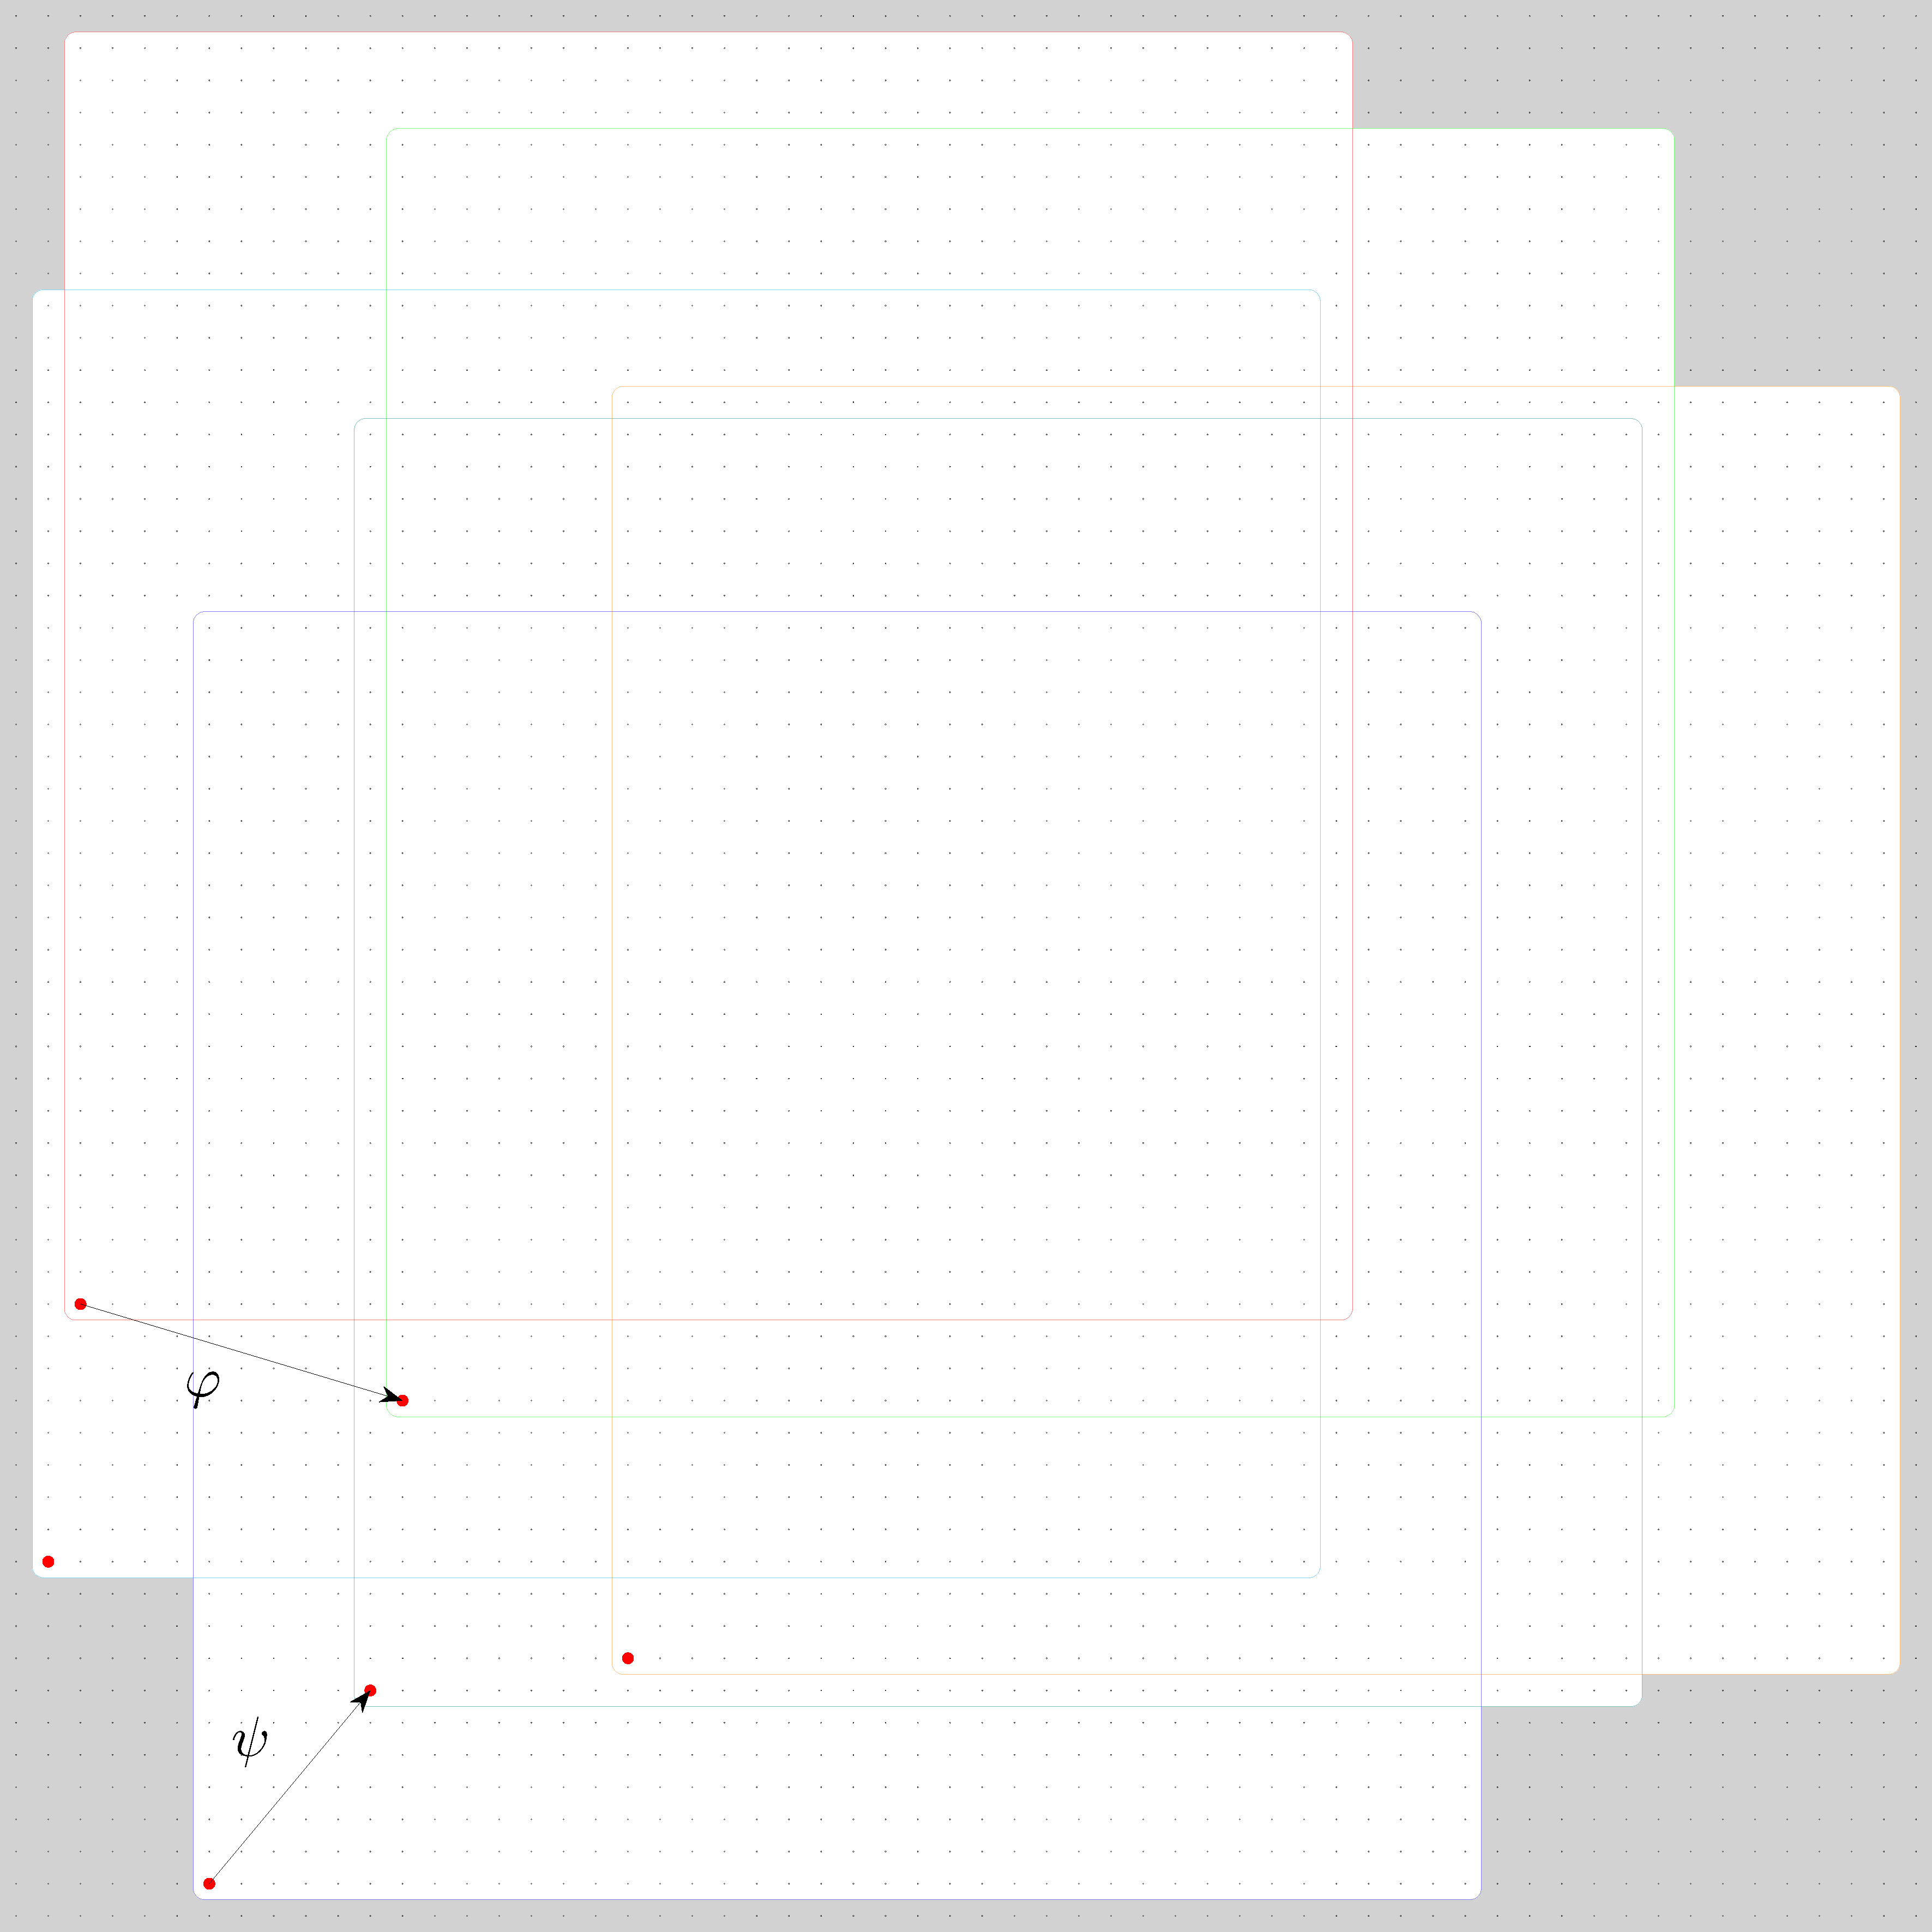
\includegraphics[width=0.8\textwidth]{drawings/occurrences}
	\end{center}
	\caption{Occurrences with small approximated Hamming distance. Red points belong to $Q$.}
	\label{figure:occurrences}
\end{figure}


\begin{definition}[Periodicity]
	Consider any vector $\delta \in \Z^2$.
	We say that a string $S$ has an $\ell$-period $\delta$ when
	\[ \Ham(S + \delta, S) \le \ell. \]
\end{definition}


\begin{lemma} \label{periodicity_lemma}
	For every $u, v \in Q$, the vector $u - v$ is an $8k$-period of $P$.
	\begin{proof}
		$\Ham(P + u - v, P) = \Ham(P + u, P + v) \le \Ham(P + u, T) + \Ham(P + v, T) \le 4k + 4k. $
	\end{proof}
\end{lemma}


\newcommand{\Q}{\mathcal{Q}}
\begin{restatable*}{theorem}{GetPeriods}\label{get_periods}
	For a given $\ell \in \Z^+$ and a set of points $U \subseteq [\ell + 1]^2$, such that $|U| > 12\ell$, there exist $s, t, s', t' \in U$, such that the following conditions hold for $w = t - s$ and $w' = t' - s'$:
	\begin{itemize}
		\item $0 < |w||w'| = \O(\ell^2 / |U|)$,
		\item $|\sin \alpha| \ge \frac{1}{2}$ where $\alpha$ is the angle between $w$ and $w'$,
		\item $w, w', -w, -w'$ are all contained in different \textbf{quadrants}, defined as
			\eq{
				\Q_1 &= (0, +\infty) \times [0, +\infty), \\
				\Q_2 &= (-\infty, 0] \times (0, +\infty), \\
				\Q_3 &= (-\infty, 0) \times (-\infty, 0], \\
				\Q_4 &= [0, +\infty) \times (-\infty, 0).
			}
	\end{itemize}
	Such $w, w'$ can be found in $\tO(|U|)$ operations.
\end{restatable*}
\begin{proof} See \Cref{get_periods_proof}. \end{proof}

We run the algorithm from \Cref{get_periods} on the set $Q$ (where $\ell = n - m \le m / 2$, thus $|Q| > 6m + m^2/k \ge 12\ell$).
Amongst $w, w', -w, -w'$ we select the vector belonging to $\Q_4$ and denote it with $\phi$.
Similarly, we select the vector belonging to $\Q_1$ and denote it with $\psi$.
By \Cref{periodicity_lemma} the vectors $\phi$ and $\psi$ are $\O(k)$-periods of $P$.
We will refer to those vectors throughout the rest of the description.
Note that because $|Q| > 6m + m^2 / k$, we have $0 \le \phi \times \psi \le |\phi||\psi| = \O(\min\set{m, k})$.
The construction of $\phi$ and $\psi$ is illustrated in \Cref{figure:occurrences}.

\begin{definition}[Lattice congruency]\label{lattice_congruency}
	We define $\L = \set{s\phi + t\psi : s, t \in \Z}$.
	We say that two vectors $u, v \in \Z^2$ are \textbf{lattice-congruent}, denoted $u \equiv v$, when $u - v \in \L$.
\end{definition}


\begin{lemma} \label{lattice_base}
	There exists a set of points $\Gamma \subseteq \Z^2$ such that $|\Gamma| = \O(\min\set{m, k})$ and every point $u \in \Z^2$ is lattice-congruent to exactly one point $\gamma \in \Gamma$.
	\begin{proof}
		Let $p = \set{s\phi + t\psi : s \in [0, 1), t \in [0, 1)}$.
		We construct $\Gamma = p \cap \Z^2$.
		By Pick's Theorem, a simple polygon with integer vertices contains $\O(A)$ integer points in the interior or on the boundary, where $A$ denotes its area.
		Observe that the points in $\Gamma$ are contained in a parallelogram with vertices $(0, 0), \phi, \phi + \psi, \psi$.
		Since its area is $\phi \times \psi = \O(\min\set{m, k})$, we get $|\Gamma| = \O(\min\set{m, k})$.
		
		Now consider any point $u \in \Z^2$.
		There exist some unique values $s, t \in [0, 1)$ and $s', t' \in \Z$, such that
		$u = (s + s') \phi + (t + t') \psi$.
		It is easy to see that
		$u \equiv s\phi + t\psi$ and $s\phi + t\psi \in \Gamma$.
	\end{proof}
\end{lemma}


\begin{figure}[!t]
	\begin{center}
		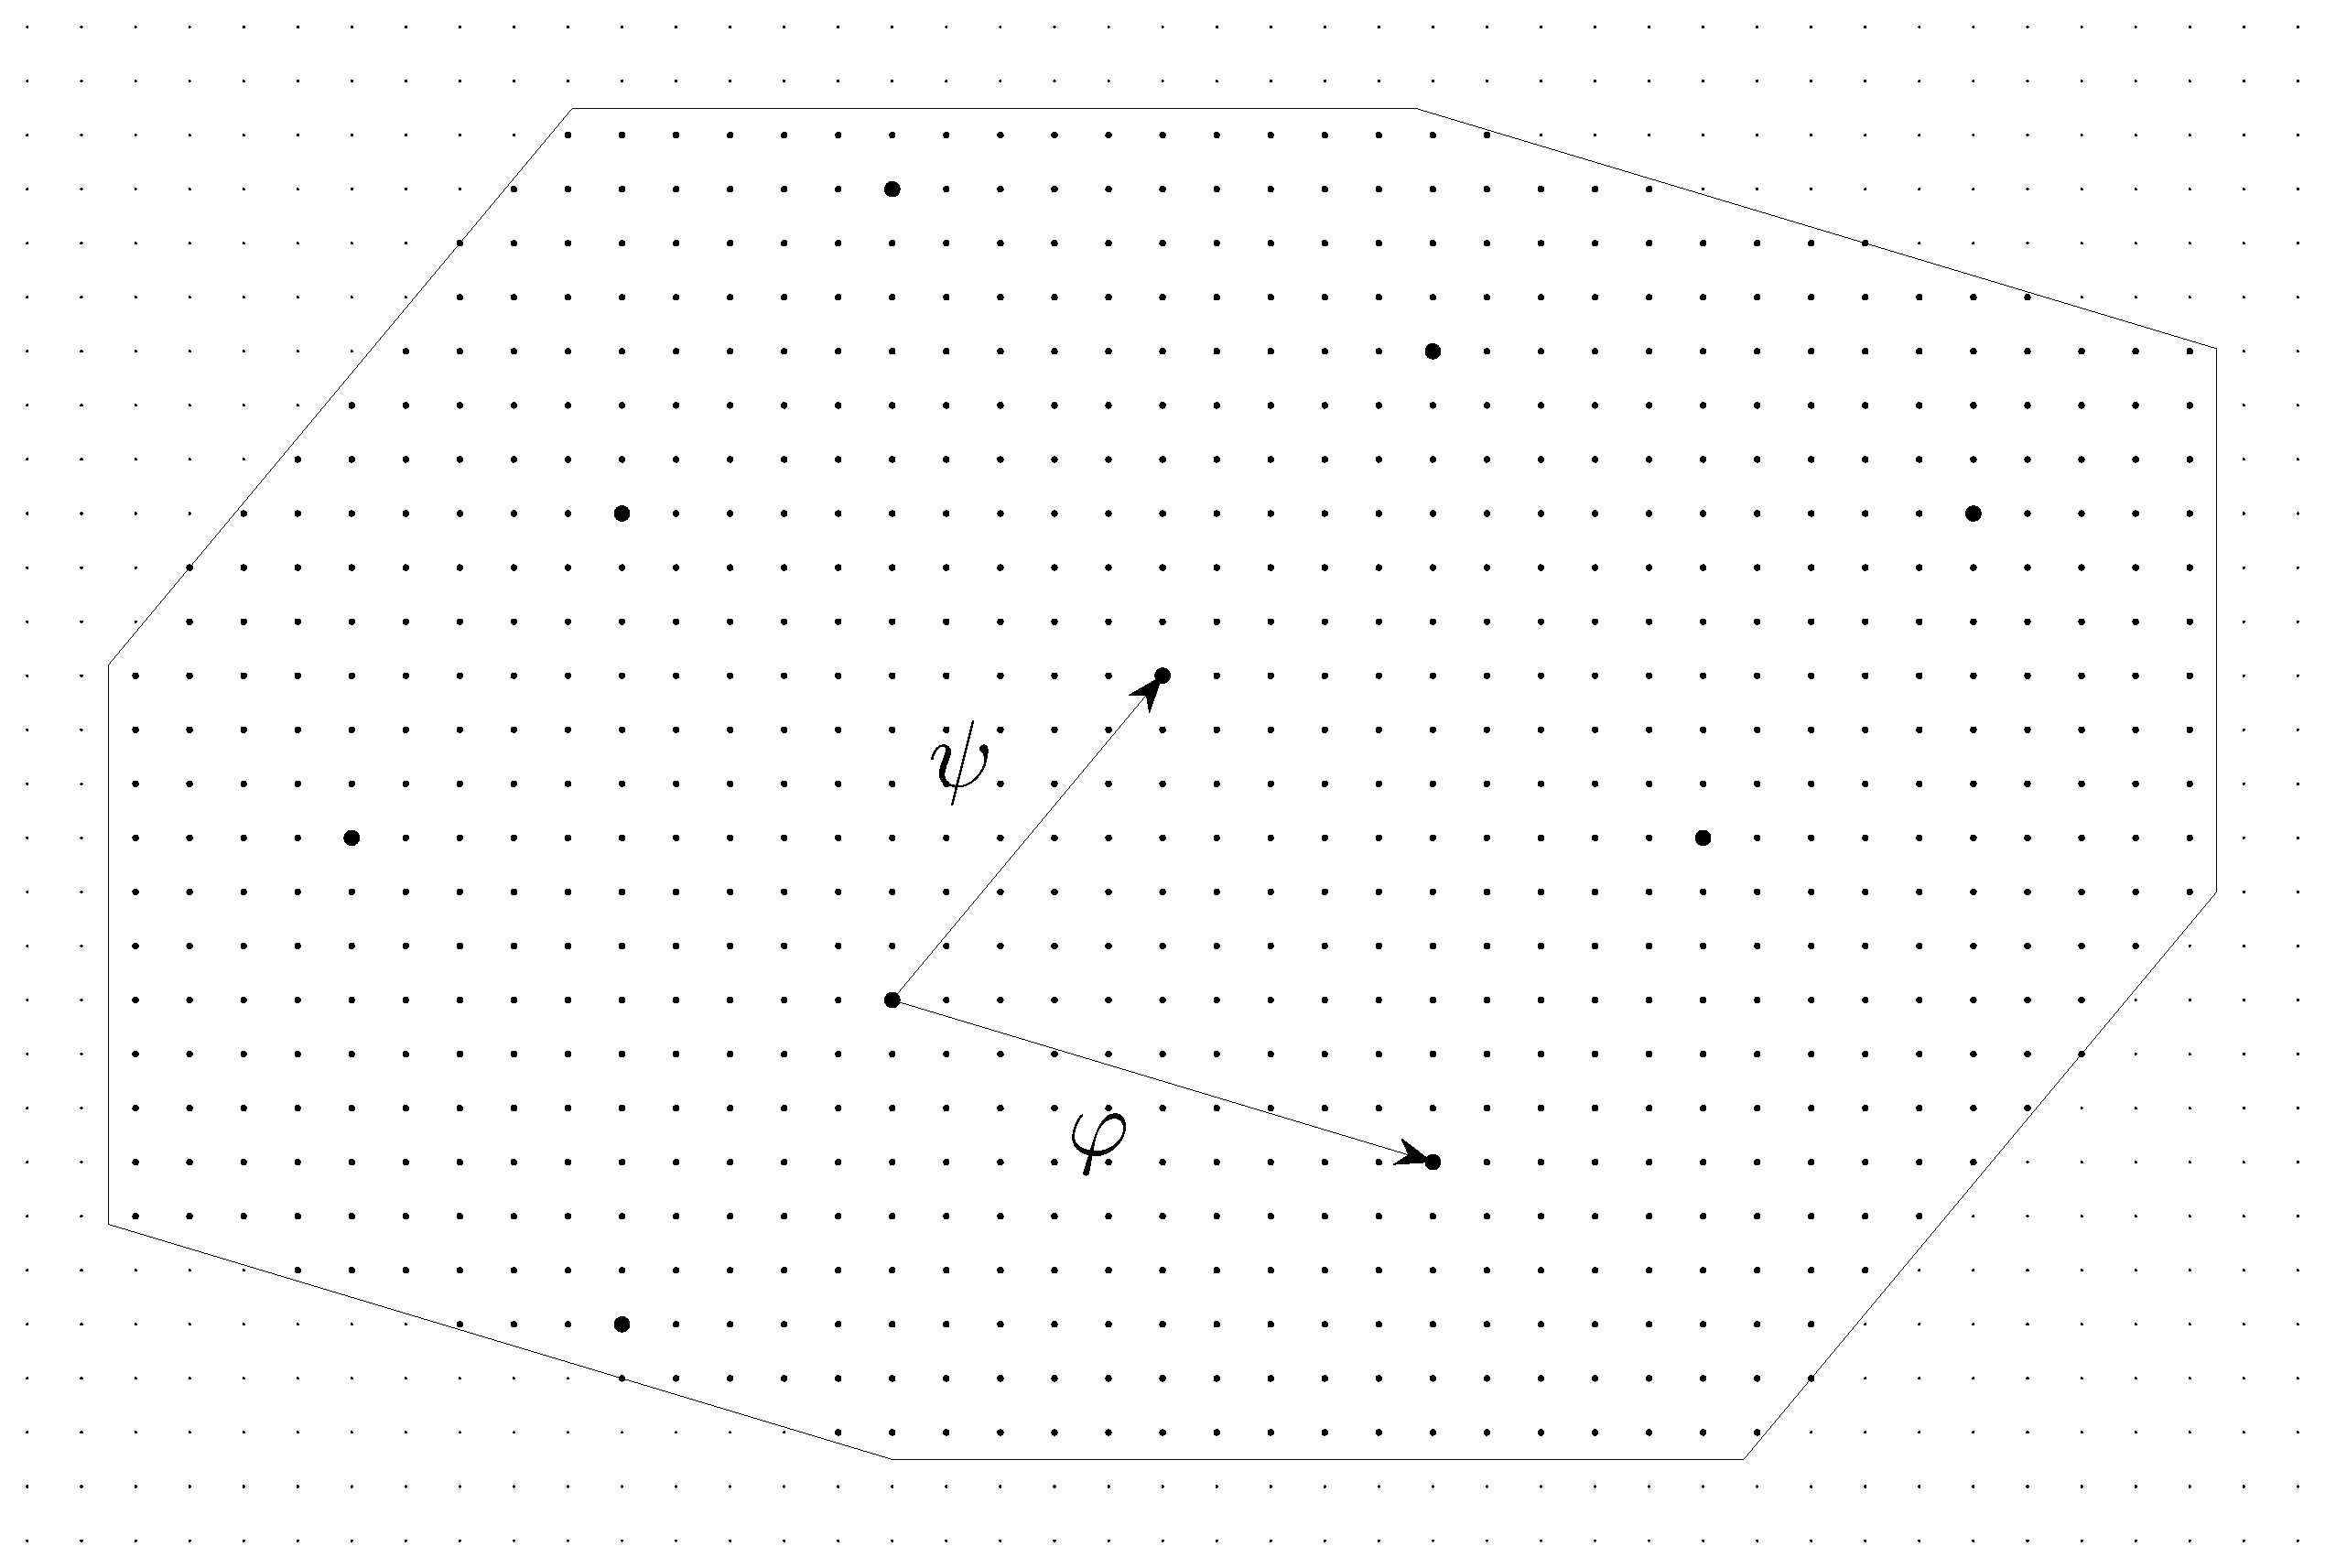
\includegraphics[width=0.8\textwidth]{drawings/parquet}
	\end{center}
	\caption{All the points in the polygon form a parquet and the red points form a subparquet.}
	\label{figure:parquet}
\end{figure}


\begin{definition}[Parquet]\label{parquet_definition}
	We call a set $U \subseteq \Z^2$ a \textbf{parquet} when there exist some values $x_0, x_1, y_0, y_1, \phi_0, \phi_1, \psi_0, \psi_1 \in \Z$, which we will call its \textbf{signature}, such that
	\[ U = [x_0, x_1] \times [y_0, y_1] \cap \set{u : u \in \Z^2, \h{u} \in [\phi_0, \phi_1], \s{u} \in [\psi_0, \psi_1]}. \]
	See \Cref{figure:parquet} for an illustration.
	\begin{enumerate}[a)]
		\item If additionally $x_1 - x_0 + 1 \ge |\x{\phi}| + |\x{\psi}|$ and $y_1 - y_0 + 1 \ge |\y{\phi}| + |\y{\psi}|$, then $U$ is a \textbf{spacious} parquet.
		\item If additionally $x_0, y_0 = -\infty$ and $x_1, y_1 = +\infty$, then $U$ is a \textbf{simple} parquet.
	\end{enumerate}
	Note that every simple parquet is spacious.
\end{definition}


\begin{definition}[Subparquet]\label{subparquet_definition}
	We call a set $V \subseteq \Z^2$ a \textbf{subparquet} when there exists a parquet $U$ and a point $\gamma \in \Z^2$ such that
	\[ V = \set{u : u \in U, u \equiv \gamma}.\]
	This is also illustrated in \Cref{figure:parquet}.
	A signature of $V$ consists of a signature of $U$ and the vector $\gamma$.
	We call $V$ a spacious/simple subparquet when there exists $U$ which is (correspondingly) a spacious/simple parquet.
	We say that $V$ is lattice-congruent to some $v \in \Z^2$ (denoted as $V \equiv v$) when $v \equiv \gamma$.
	We similarly define the lattice congruency between two subparquets.
\end{definition}


\begin{definition}[Parquet string]\label{parquet_string_definition}
	We call a string $S$ a spacious/simple (sub-)parquet string when $\d{S}$ is a spacious/simple (sub-)parquet.
\end{definition}


\begin{restatable*}{theorem}{ParquetDecomposition}\label{parquet_decomposition}
	A given spacious/simple parquet string $R$ with $\O(k)$-periods $\phi$ and $\psi$ can be partitioned in time $\tO(|\d{R}| + k)$ into $\O(k)$ monochromatic spacious/simple subparquet strings, correspondingly.
\end{restatable*}
\begin{proof} See \Cref{parquet_decomposition_proof}. \end{proof}


Since $|\x{\phi}|, |\y{\phi}|, |\x{\psi}|, |\y{\psi}| \le n - m \le m / 2$, the $m \times m$ string $P$ is a spacious parquet string and satisfies the assumptions of \Cref{parquet_decomposition}.
We partition $P$ into a set of strings $\V$.
We then group the strings based on the single character they contain.
Specifically, for every character $\sigma \in \Sigma$ present in $P$, we construct the set $\V_\sigma = \set{V : V \in \V, \getchar{V} = \sigma}$ (recall that we defined $\getchar{\cdot}$ in \cref{string_definition}).

\begin{restatable*}{theorem}{SparseAlgo}\label{sparse_algo}
	For a given set of monochromatic simple subparquet strings $\S$ we can calculate
	\[ \sum_{S \in \S} \Ham(P + q, S) \]
	for every $q \in Q$ in total time $\tO(m^2 + \sum_{S \in \S} |\V_{\getchar{S}}|)$, assuming that the sets $\d{S}$ for $S \in \S$ are some pairwise disjoint subsets of $\d{T}$.
\end{restatable*}
\begin{proof} See \Cref{subparquet_convolution_proof}. \end{proof}

% TEXT DECOMPOSITION
\subsection{Text decomposition}
Because the text is not necessarily periodic, we unfortunately cannot use the same approach as for the pattern.
In this section we show how to decompose $T$ using a similar, but more nuanced method.


\newcommand{\Ta}{T_\mathbf{a}}
\begin{definition}[Active text]
	We define the \textbf{active text} $\Ta$ as the restriction of $T$ to
	\[ \bigcup_{q \in Q} \d{P + q}. \]
	In \Cref{figure:occurrences} the points in the white area form the set $\d{\Ta}$.
\end{definition}

\begin{observation}
	$\Ham(P + q, T) = \Ham(P + q, \Ta)$ for every $q \in Q$.
\end{observation}

\begin{definition}[Peripherality]
	For every point $u \in \Z^2$ we define its \textbf{border distance} as
	$\min\set{|u - v| : v \in \Z^2 \setminus \d{\Ta}} $.
	We say that a set of points $U \subseteq \Z^2$ is $d$-\textbf{peripheral} for some $d \ge 0$, if the border distance of every $u \in U$ is not greater than $d$.
	We say that a string $S$ is $d$-peripheral when $\d{S}$ is $d$-peripheral.
\end{definition}

\begin{restatable*}{theorem}{TextDecomposition}\label{text_decomposition}
	Given any $\ell \in \Z^+$, we can partition the active text in time $\tO(m^2 + \ell k)$ into a set of $\O(\ell k)$ monochromatic simple subparquet strings and an $\O(m / \ell)$-peripheral string.
\end{restatable*}
\begin{proof} See \Cref{text_decomposition_proof}. \end{proof}

\paragraph{Warm-up algorithm.}
An immediate consequence of \Cref{text_decomposition} is that we can partition the active text into $\O(mk)$ monochromatic simple subparquet strings.
We can construct such a partitioning by substituting a large enough value $\ell = \Theta(m)$, such that the obtained $\O(m / \ell)$-peripheral string is in fact $0$-peripheral, and thus empty.
If we denote the resulting set of monochromatic simple subparquet strings as $\S$, for every $q \in Q$ we have
\[ \Ham(P + q, \Ta) = \sum_{S \in \S} \Ham(P + q, S).\]
By \Cref{sparse_algo}, we can calculate $\sum_{S \in \S} \Ham(P + q, S)$ for every $q \in Q$ in time $\tO(m^2 + mk^{2})$,
since $\sum_{S \in \S} |\V_{\getchar{S}}| \le |\S| |\V| = \O(mk \cdot k)$.
This yields us a complete $\tO((m^2 + mk^2)n^2/m^2)$ solution for the \HD problem, which for $k = \O(m ^ {1/2})$, works in optimal time $\tO(n^2)$.

\paragraph{Main algorithm.}
To obtain the promised $\tO(m^2 + mk^{5/4})$ complexity, we partition the active text using the algorithm from \Cref{text_decomposition} with $\ell = mk^{-3/4}$.
We obtain a set of $\O(mk^{1/4})$ simple subparquet strings $\S$, and a $\O(k^{3 / 4})$-peripheral string $F$.
For every $q \in Q$ we then have
\[ \Ham(P + q, \Ta) = \Ham(P + q, F) + \sum_{S \in \S} \Ham(P + q, S).\]
By \Cref{sparse_algo}, we can calculate $\sum_{S \in \S} \Ham(P + q, S)$ for every $q \in Q$ in time $\tO(m^2 + mk^{5/4})$,
since similarly we have $\sum_{S \in \S} |\V_{\getchar{S}}| \le |\S| |\V| = \O(mk^{5/4})$.
In \Cref{periphery_section} we will introduce \Cref{dense_algo}, which states that for a $d$-peripheral string $F$, we can calculate $\Ham(P + q, F)$ for every $q \in Q$ in total time $\tO(m^2 + mdk^{1/2})$.
By substituting $d = \O(k^{3/4})$, we get the total complexity of $\tO(m^2 + mk^{5/4})$ as promised.


% BORDER PROXIMITY
\subsection{Text periphery}\label{periphery_section}
\begin{figure}[!t]
	\begin{center}
		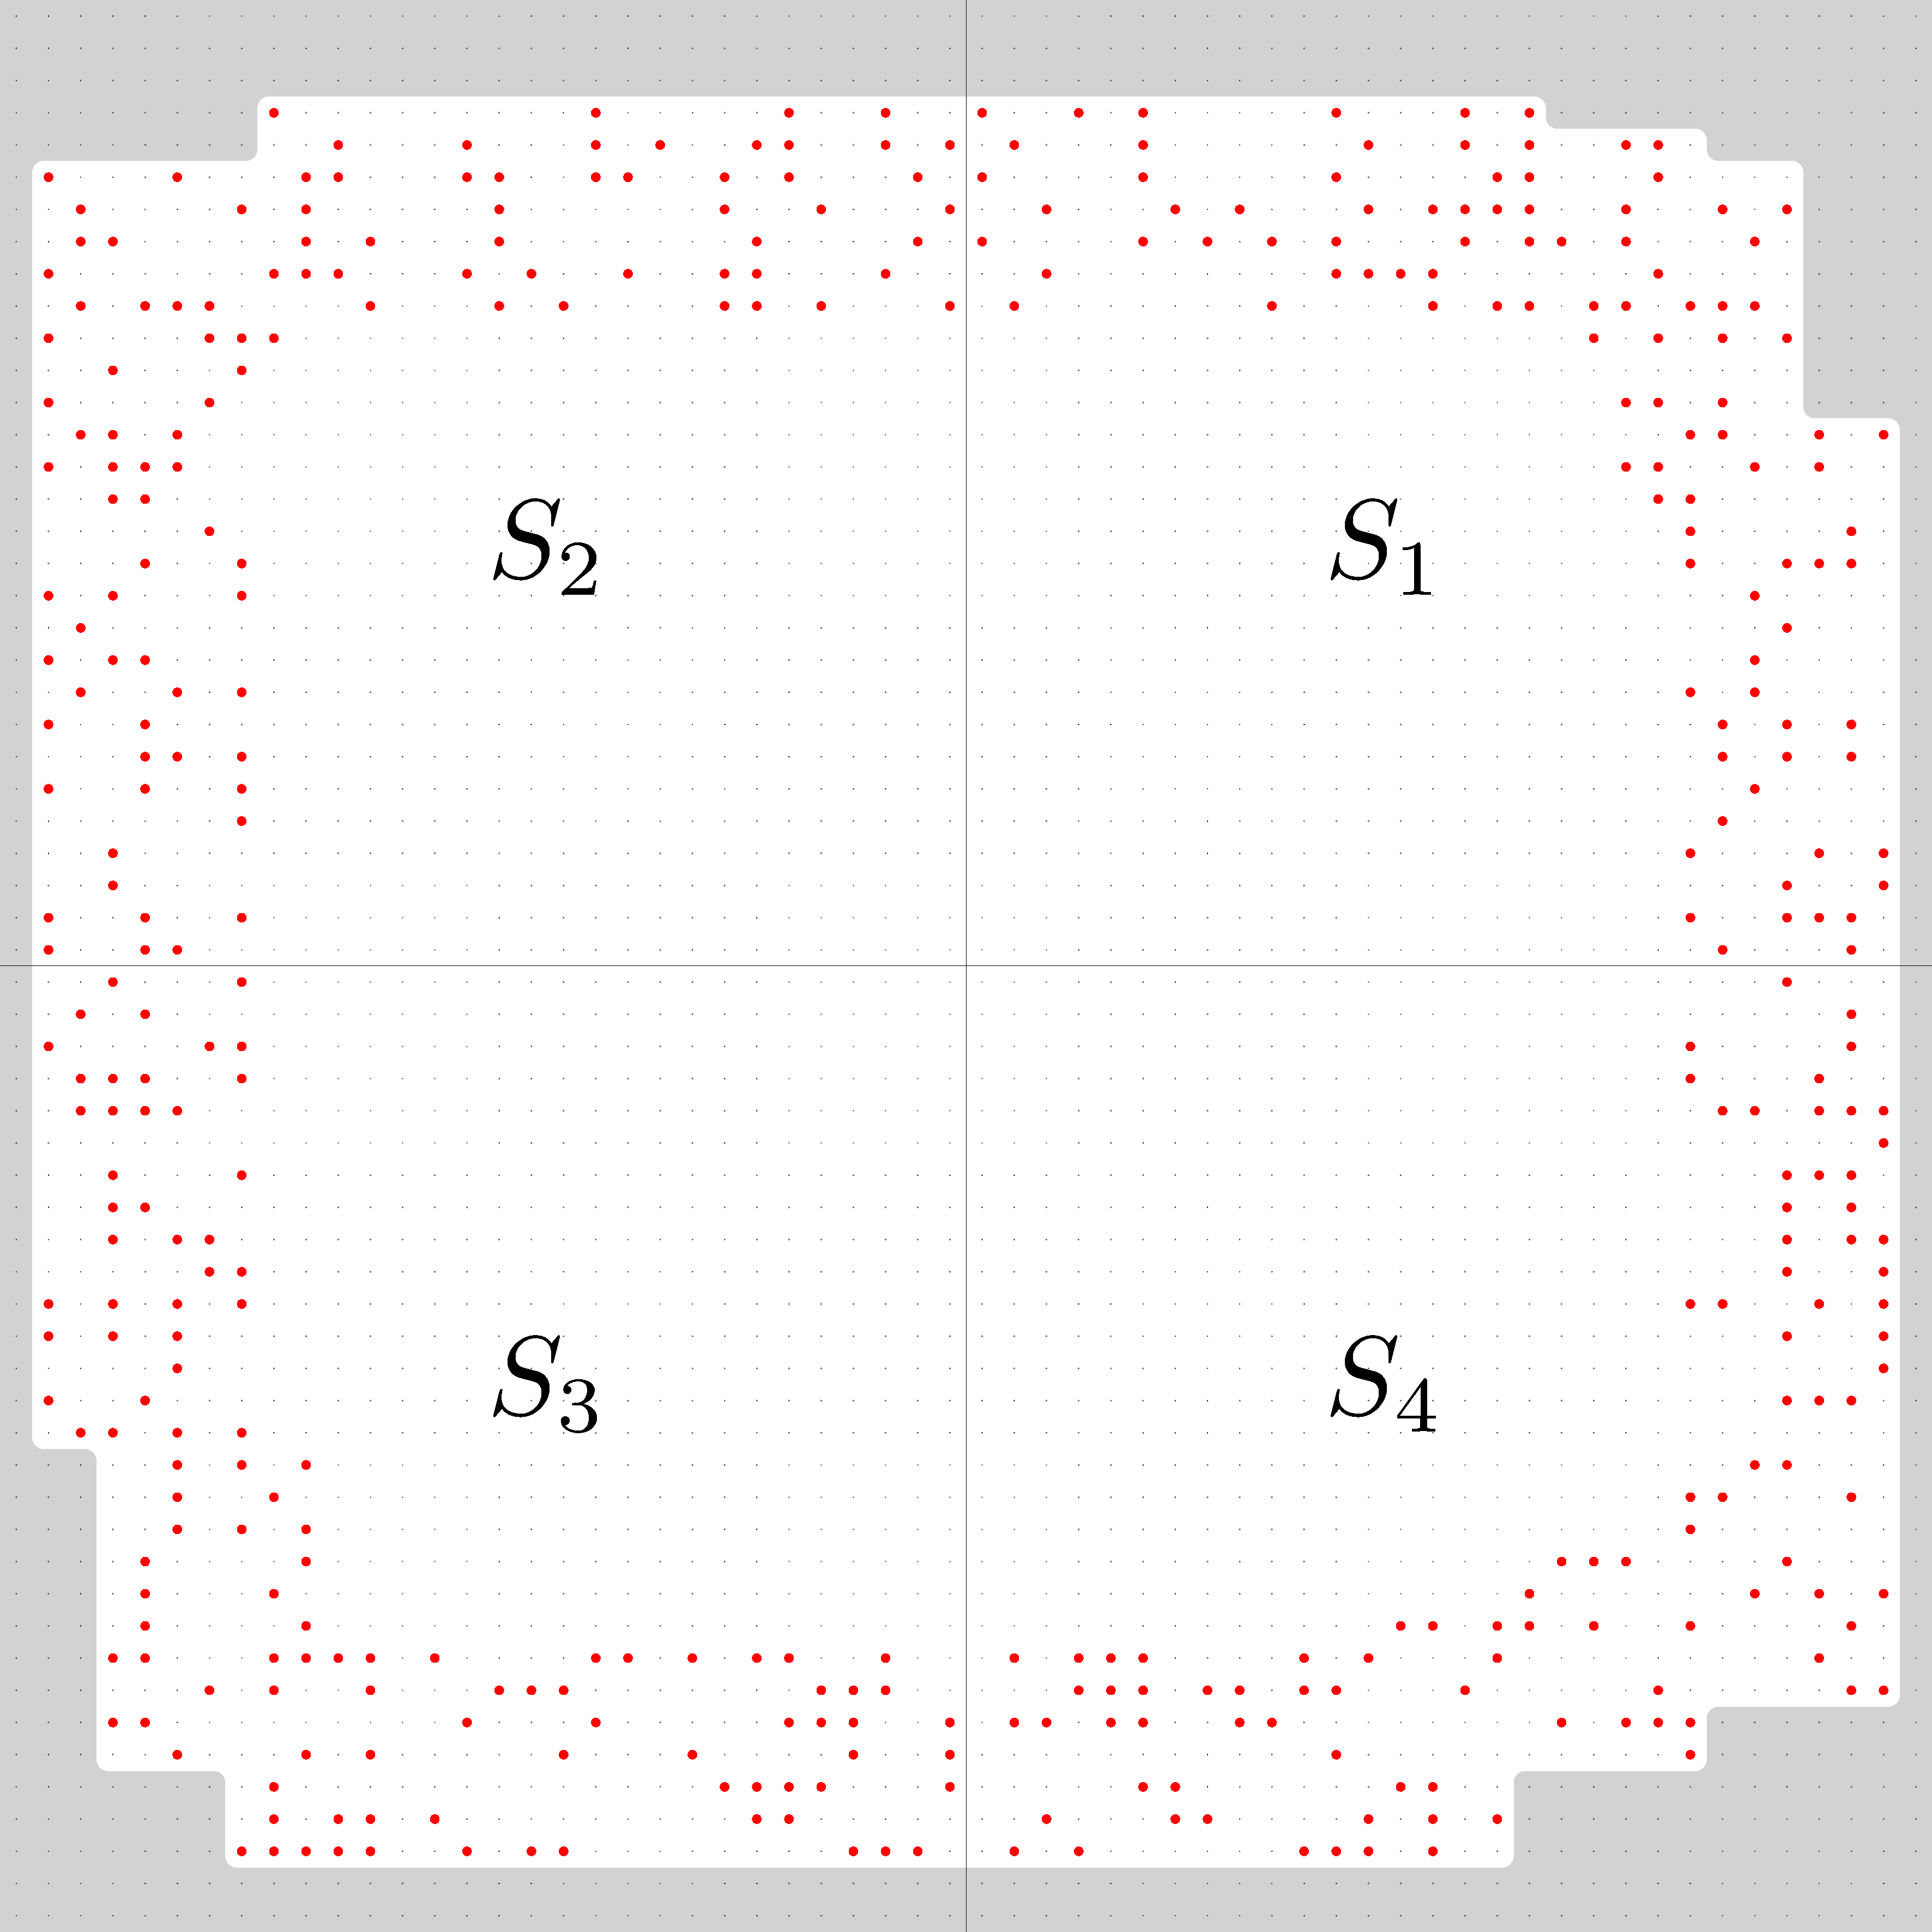
\includegraphics[width=0.8\textwidth]{drawings/quarter_split}
	\end{center}
	\caption{Construction of $S_1, \dots, S_4$. The red points represent $\d{S}$.}
	\label{figure:quarter_split}
\end{figure}
In this section we explore the properties of peripheral strings.
We consider any $d > 0$ and a non-empty $d$-peripheral string $S$, such that $\d{S} \subseteq \d{\Ta}$.
We define a partitioning of $S$ into strings $S_1, \dots, S_4$, by splitting it through the middle with a horizontal and vertical line. 
Specifically
\begin{itemize}
	\item $S_1$ is the restriction of $S$ to $\set{n / 2, \dots, n - 1} \times \set{n / 2, \dots, n - 1}$ (upper right quarter),
	\item $S_2$ is the restriction of $S$ to $\set{0, \dots, n / 2 - 1} \times \set{n / 2, \dots, n - 1}$ (upper left quarter),
	\item $S_3$ is the restriction of $S$ to $\set{0, \dots, n / 2 - 1} \times \set{0, \dots, n / 2 - 1}$ (lower left quarter),
	\item $S_4$ is the restriction of $S$ to $\set{n / 2, \dots, n - 1} \times \set{0, \dots, n / 2 - 1}$ (lower right quarter).
\end{itemize}
See \Cref{figure:quarter_split} for an illustration.
We will now demonstrate some characteristics of $S_1$, and by symmetry, generalize them to $S$.

\begin{lemma} \label{border_lemma}
	Assuming $d \le m/4$, there does not exist $u \in S_1$ and $v \in T_a$ such that $\x{v} - \x{u} \ge d$ and $\y{v} - \y{u} \ge d$.
	\begin{proof}
		Assume the contrary.
		Since $u \in S_1$, the border distance of $u$ is at most $d$, so there exists $w \in \Z^2 \setminus \d{\Ta}$, such that
		$\x{u} - d \le \x{w} \le \x{u} + d$ and
		$\y{u} - d \le \y{w} \le \y{u} + d$.
		Since $v \in T_a$, there exists $q \in Q$ such that $v \in [m]^2 + q$.
		We have
		\[ \x{w} \ge \x{u} - d \ge n / 2 - m / 4 \ge n - m > \x{q} \]
		and
		\[ \x{w} \le \x{u} + d \le \x{v} \le \x{q} + m - 1. \]
		Similarly we can show that $\y{q} \le \y{w} \le \y{q} + m - 1$, and thus $w \in [m]^2 + q$.
		Since $[m]^2 + q \subseteq \d{\Ta}$ and $w \not \in \Ta$, we get a contradiction.
	\end{proof}
\end{lemma}

We now introduce two major theorems regarding peripheral strings, the first of which is proven in the next section (\ref{sigma_border_proof}):

\begin{restatable*}{theorem}{SigmaBorder}\label{sigma_border}
	We can calculate $\Ham(P + q, S)$ for every $q \in Q$ in total time $\tO(m^2 + md |\Sigma|)$, where $|\Sigma|$ is the number of different characters present in both $P$ and $S$.
\end{restatable*}

\begin{theorem}\label{dense_algo}
	We can calculate $\Ham(P + q, S)$ for every $q \in Q$ in total time $\tO(m^2 + mdk^{1/2})$.
\end{theorem}
\begin{proof}
	Recall the construction of the sets $\V_\sigma$ described in \Cref{periodicity_section}.
	We define $\sigma \in \Sigma$ to be a \textbf{frequent} character if $|\V_\sigma| \ge \sqrt{k}$ and if $|\V_\sigma| < \sqrt{k}$, we call it an \textbf{infrequent} character.
	We partition $S$ into two strings $F$ and $I$, based on character frequency,
	so that $F$ consists of only the frequent characters and $I$ consists of only the infrequent ones.
	For every $q \in Q$ we then have 
	\[\Ham(P + q, S) = \Ham(P + q, F) + \Ham(P + q, I).\]
	
	Observe that the number of different frequent characters is $\O(\sqrt{k})$, and thus, by \Cref{sigma_border}, we can calculate $\Ham(P + q, F)$ for every $q \in Q$ in total time $\tO(m^2 + mdk^{1/2})$, since $F$ is $d$-peripheral. 
	
	We partition $I$ into $|\d{I}|$ strings, one per every $u \in I$.
	Specifically, let $I_u$ be the restriction of $I$ to $\set{u}$ for every $u \in I$.
	We have $\Ham(P + q, I) = \sum_{u \in I} \Ham(P + q, I_u)$ for every $q \in Q$.
	By \Cref{subparquet_definition}, $I_u$ are simple subparquet strings, and thus, we can by \Cref{sparse_algo} calculate the results in $\tO(m^2 + \sum_{u \in I} |\V_{I(u)}|)$.
	Since $I(u)$ is an infrequent character for every $u \in I$, we have $|\V_{I(u)}| < k^{1/2}$ for every $u \in I$.
	By \Cref{area_bound} we have $|\d{I}| = \O(md)$, and thus the total complexity is $\tO(m^2 + mdk^{1/2})$.
\end{proof}

\subsubsection{Peripheral convolution} \label{sigma_border_proof}

This section serves as the proof of the theorem we just used to prove \Cref{dense_algo}:

\SigmaBorder

We base our approach on the simple method of calculating the Hamming distance by running an instance of FFT for each unique character.
We will again utilize partitioning to reduce the problem to some smaller ones and then solve them naively.
We will take advantage of the fact that the points close to the border can overlap only with a small subset of points from the pattern when considering the occurrences fully contained in the active text.

Recall that 
$\Ham(P + q, S) = \Ham(P + q, S_1) + \dots + \Ham(P + q, S_4)$.
We will only show how to calculate $\Ham(P + q, S_1)$ for every $q \in Q$, since the other cases are symmetric.
Consider a string $P_0$, defined as the restriction of $P$ to $[m - d]^2$ and a string $P_1$, defined as the restriction of $P$ to $\d{P} \setminus \d{P_0}$.
Since the strings $P_0$ and $P_1$ partition $P$, we have
\[ \Ham(P + q, S_1) = \Ham(P_0 + q, S_1) + \Ham(P_1 + q, S_1).\]

\begin{definition}(width \& height)\label{width_and_height_definition}
	For a non-empty set $U \subseteq \Z^2$ we define its \textbf{width} as $\max\set{\x{u} - \x{v} + 1 : u, v \in U}$
	and its \textbf{height} as $\max\set{\y{u} - \y{v} + 1 : u, v \in U}$.
	For a non-empty string $R$ we define the width and height as the width and height of $\d{R}$.
\end{definition}

\begin{theorem}\label{general_fft}
	Given two non-empty strings $P$ and $T$ of widths $w_P, w_T$ and heights $h_P, h_T$, we can calculate $\Ham(P + q, T)$ for every $q \in \Z^2$, for which the result is non-zero, in total time $\tO((|\Sigma| + 1)(w_P + w_T)(h_P + h_T))$, where $|\Sigma|$ denotes the number of different characters present in both $P$ and $T$.
	\begin{proof}
		We can prove it by slightly generalizing \Cref{sigman2d}, although following the same method, and utilizing \Cref{dontcare_padding}.
	\end{proof}
\end{theorem}

From now we will assume that $d \le m / 4$, since for $d > m / 4$ we can, by \Cref{general_fft}, calculate the results in time $\tO(m^2 + m^2|\Sigma|)$, which is sufficient.


\begin{lemma}\label{border_hamming_reduction}
	$\d{P_0 + q} \cap \d{S_1} = \emptyset$ for every $q \in Q$.
	\begin{proof}
		Let us assume the contrary.
		Select any $q \in Q$ such that $\d{P_0 + q} \cap \d{S_1}$ 
		contains some point $u$ and consider the point $v = (\x{u} + d, \y{u} + d)$.
		Since $u \in [m - d]^2 + q$, we have $v \in [m]^2 + q \subseteq \d{\Ta}$, thus the points $u \in S_1$ and $v \in \Ta$ contradict \Cref{border_lemma}.
	\end{proof}
\end{lemma}

\begin{observation}\label{border_hamming_split}
	$P_1$ can be partitioned into two strings $P_2$ and $P_3$ such that the width of $P_2$ and the height of $P_3$ are equal to $d$.
\end{observation}

By \Cref{border_hamming_reduction}, $\Ham(P_0 + q, S_1) = 0$ for every $q \in Q$
and by \Cref{border_hamming_split} we have 
\[\Ham(P + q, S_1) = \Ham(P_1 + q, S_1) = \Ham(P_2 + q, S_1) + \Ham(P_3 + q, S_1) \]
for some strings $P_2$ and $P_3$ partitioning $P_1$, such that the width of $P_2$ and the height of $P_3$ are equal to $d$.
We calculate $\Ham(P_2 + q, S_1)$ and $\Ham(P_3 + q, S_1)$ for every $Q$ independently and sum the results.
We only show how to calculate $\Ham(P_2 + q, S_1)$, since the other case is symmetric.

We will now partition $S_1$.
Consider a sequence of strings $U_0, \dots, U_{\lceil n / d \rceil - 1}$, where $U_i$ is the restriction of $S_1$ to $\set{id, \dots, id + d - 1} \times [n] \cap \d{S_1}$.
For the sake of formality (since the maximum/minimum of an empty set is undefined), let $V_0, \dots, V_{\ell - 1}$ consist of all non-empty strings $U_i$, given in the increasing order of $i$.
Observe that $V_0, \dots, V_{\ell - 1}$ partition $S_1$ and their width is not greater than $d$.

\begin{figure}[!t]
	\begin{center}
		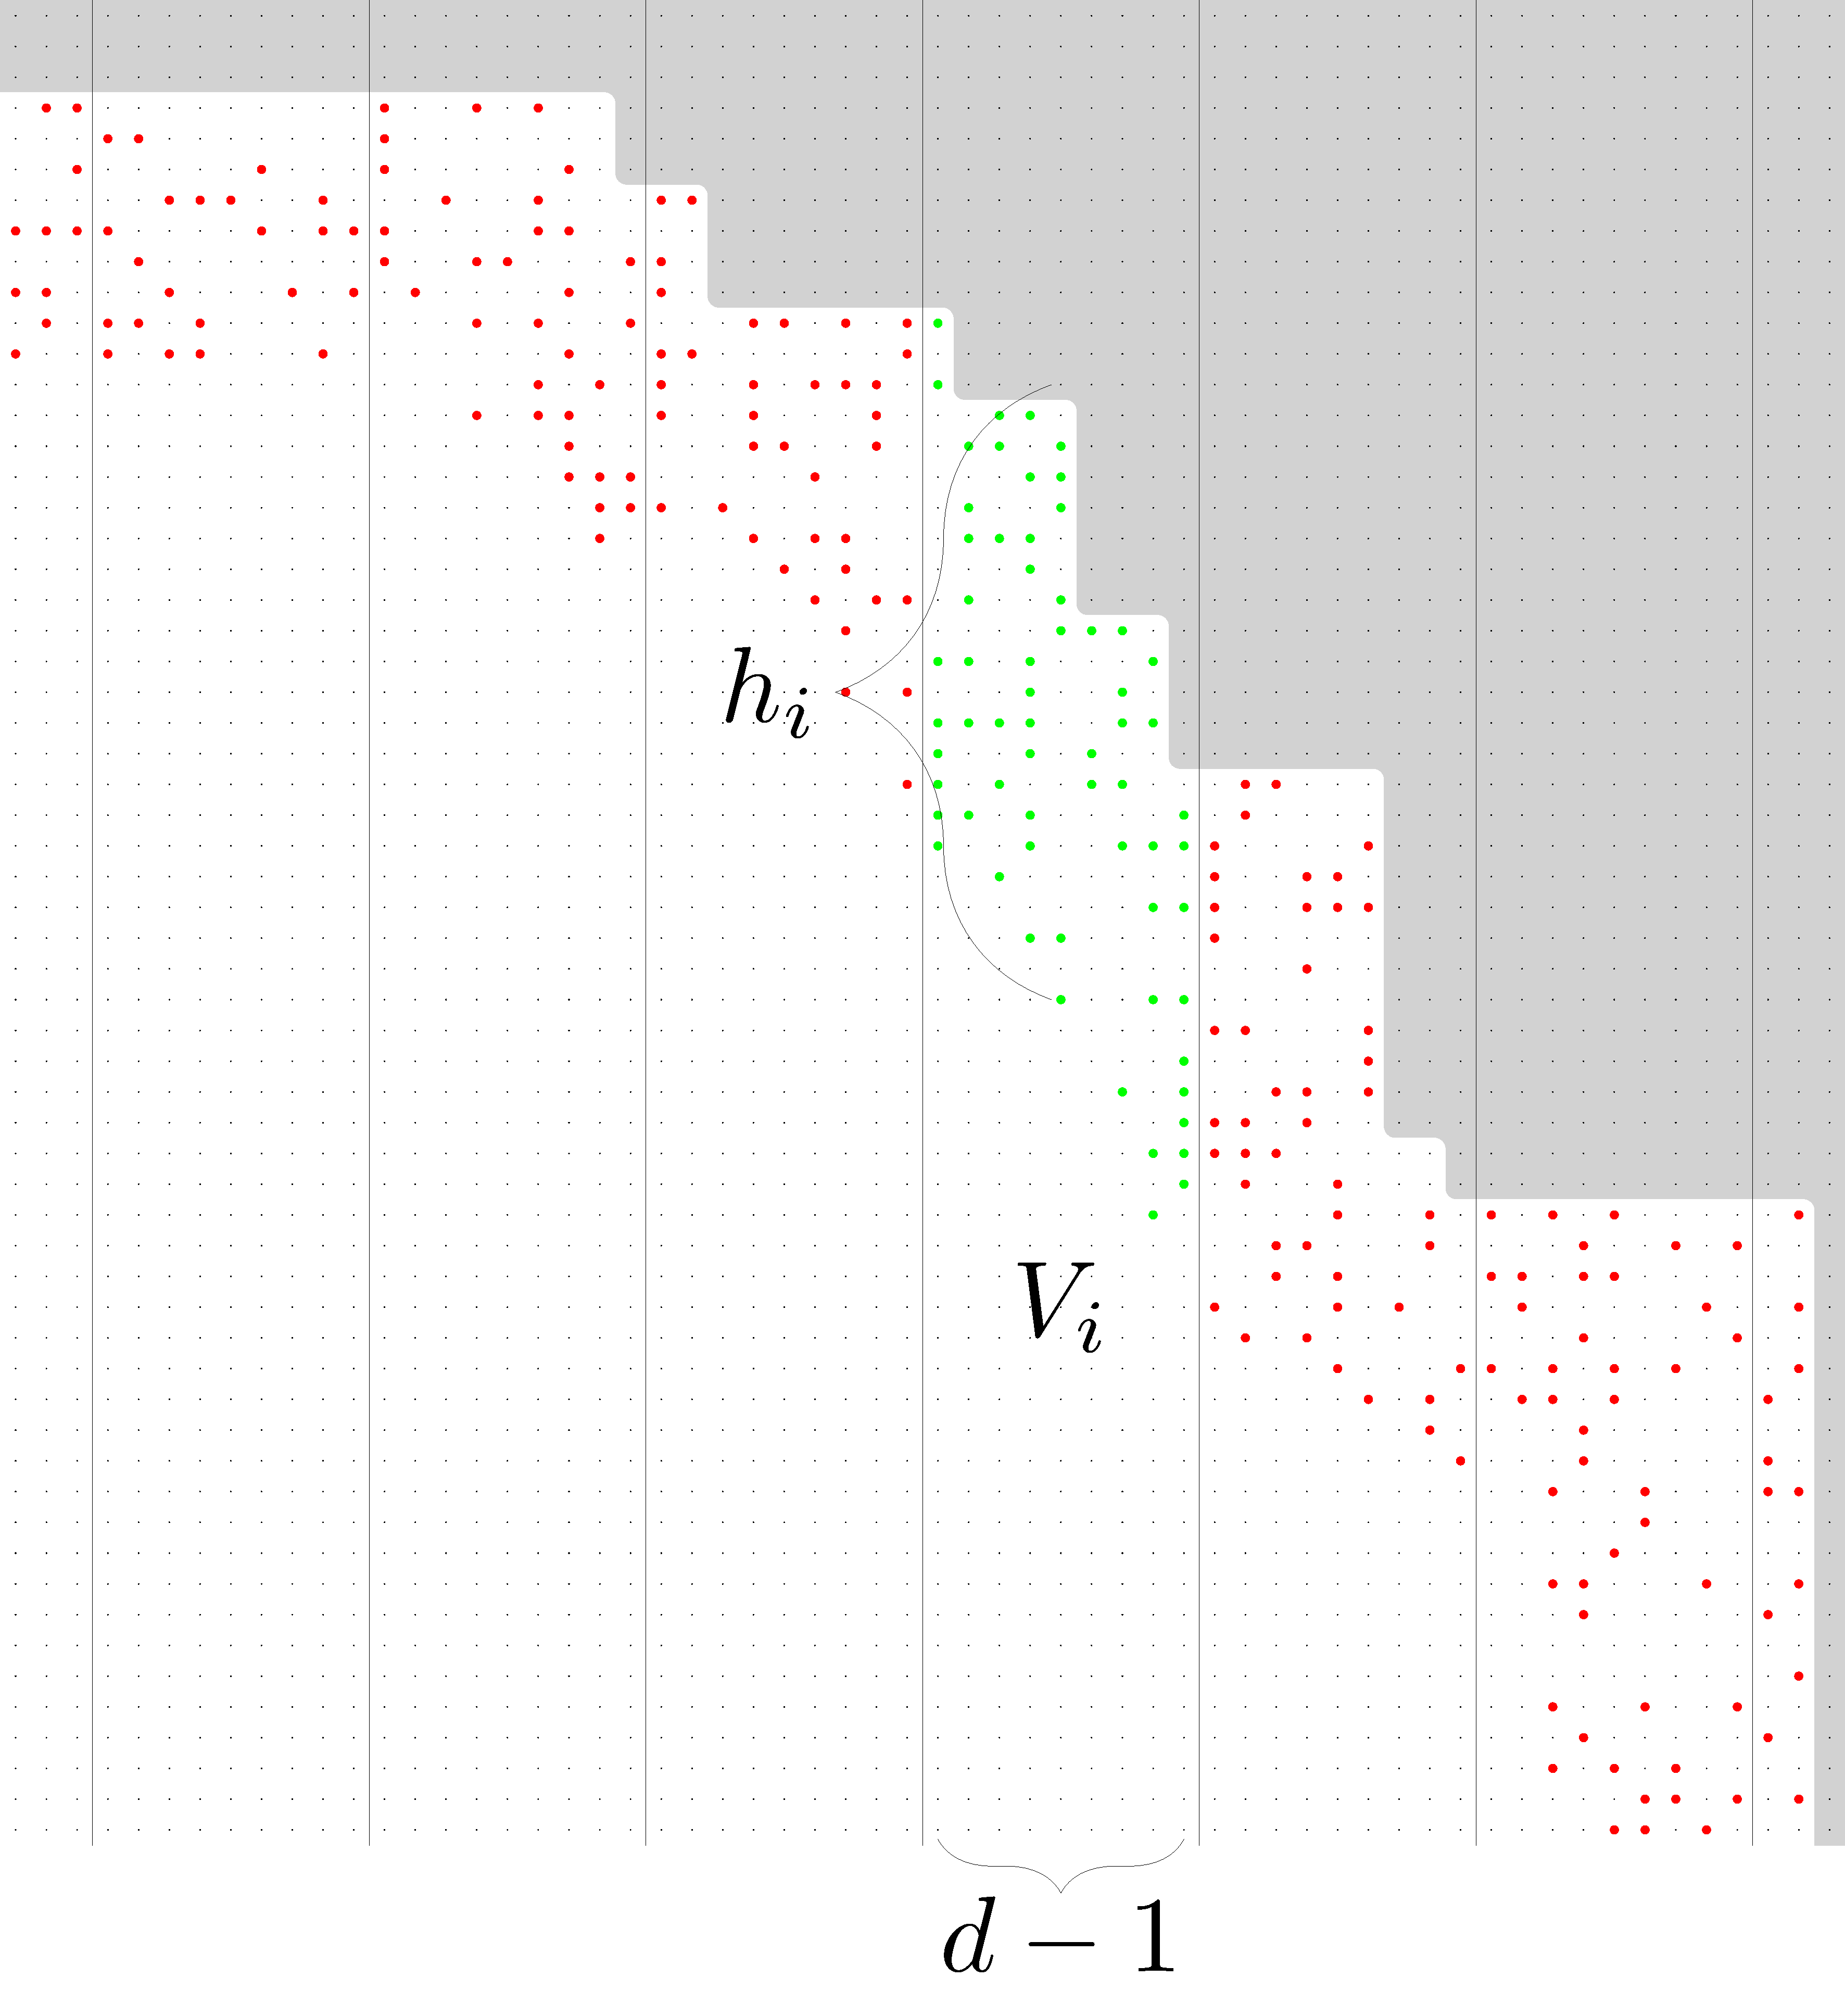
\includegraphics[width=0.8\textwidth]{drawings/periphery_decomposition}
	\end{center}
	\caption{The decomposition of $S_1$.}
	\label{figure:periphery_decomposition}
\end{figure}

\begin{figure}[!t]
	\begin{center}
		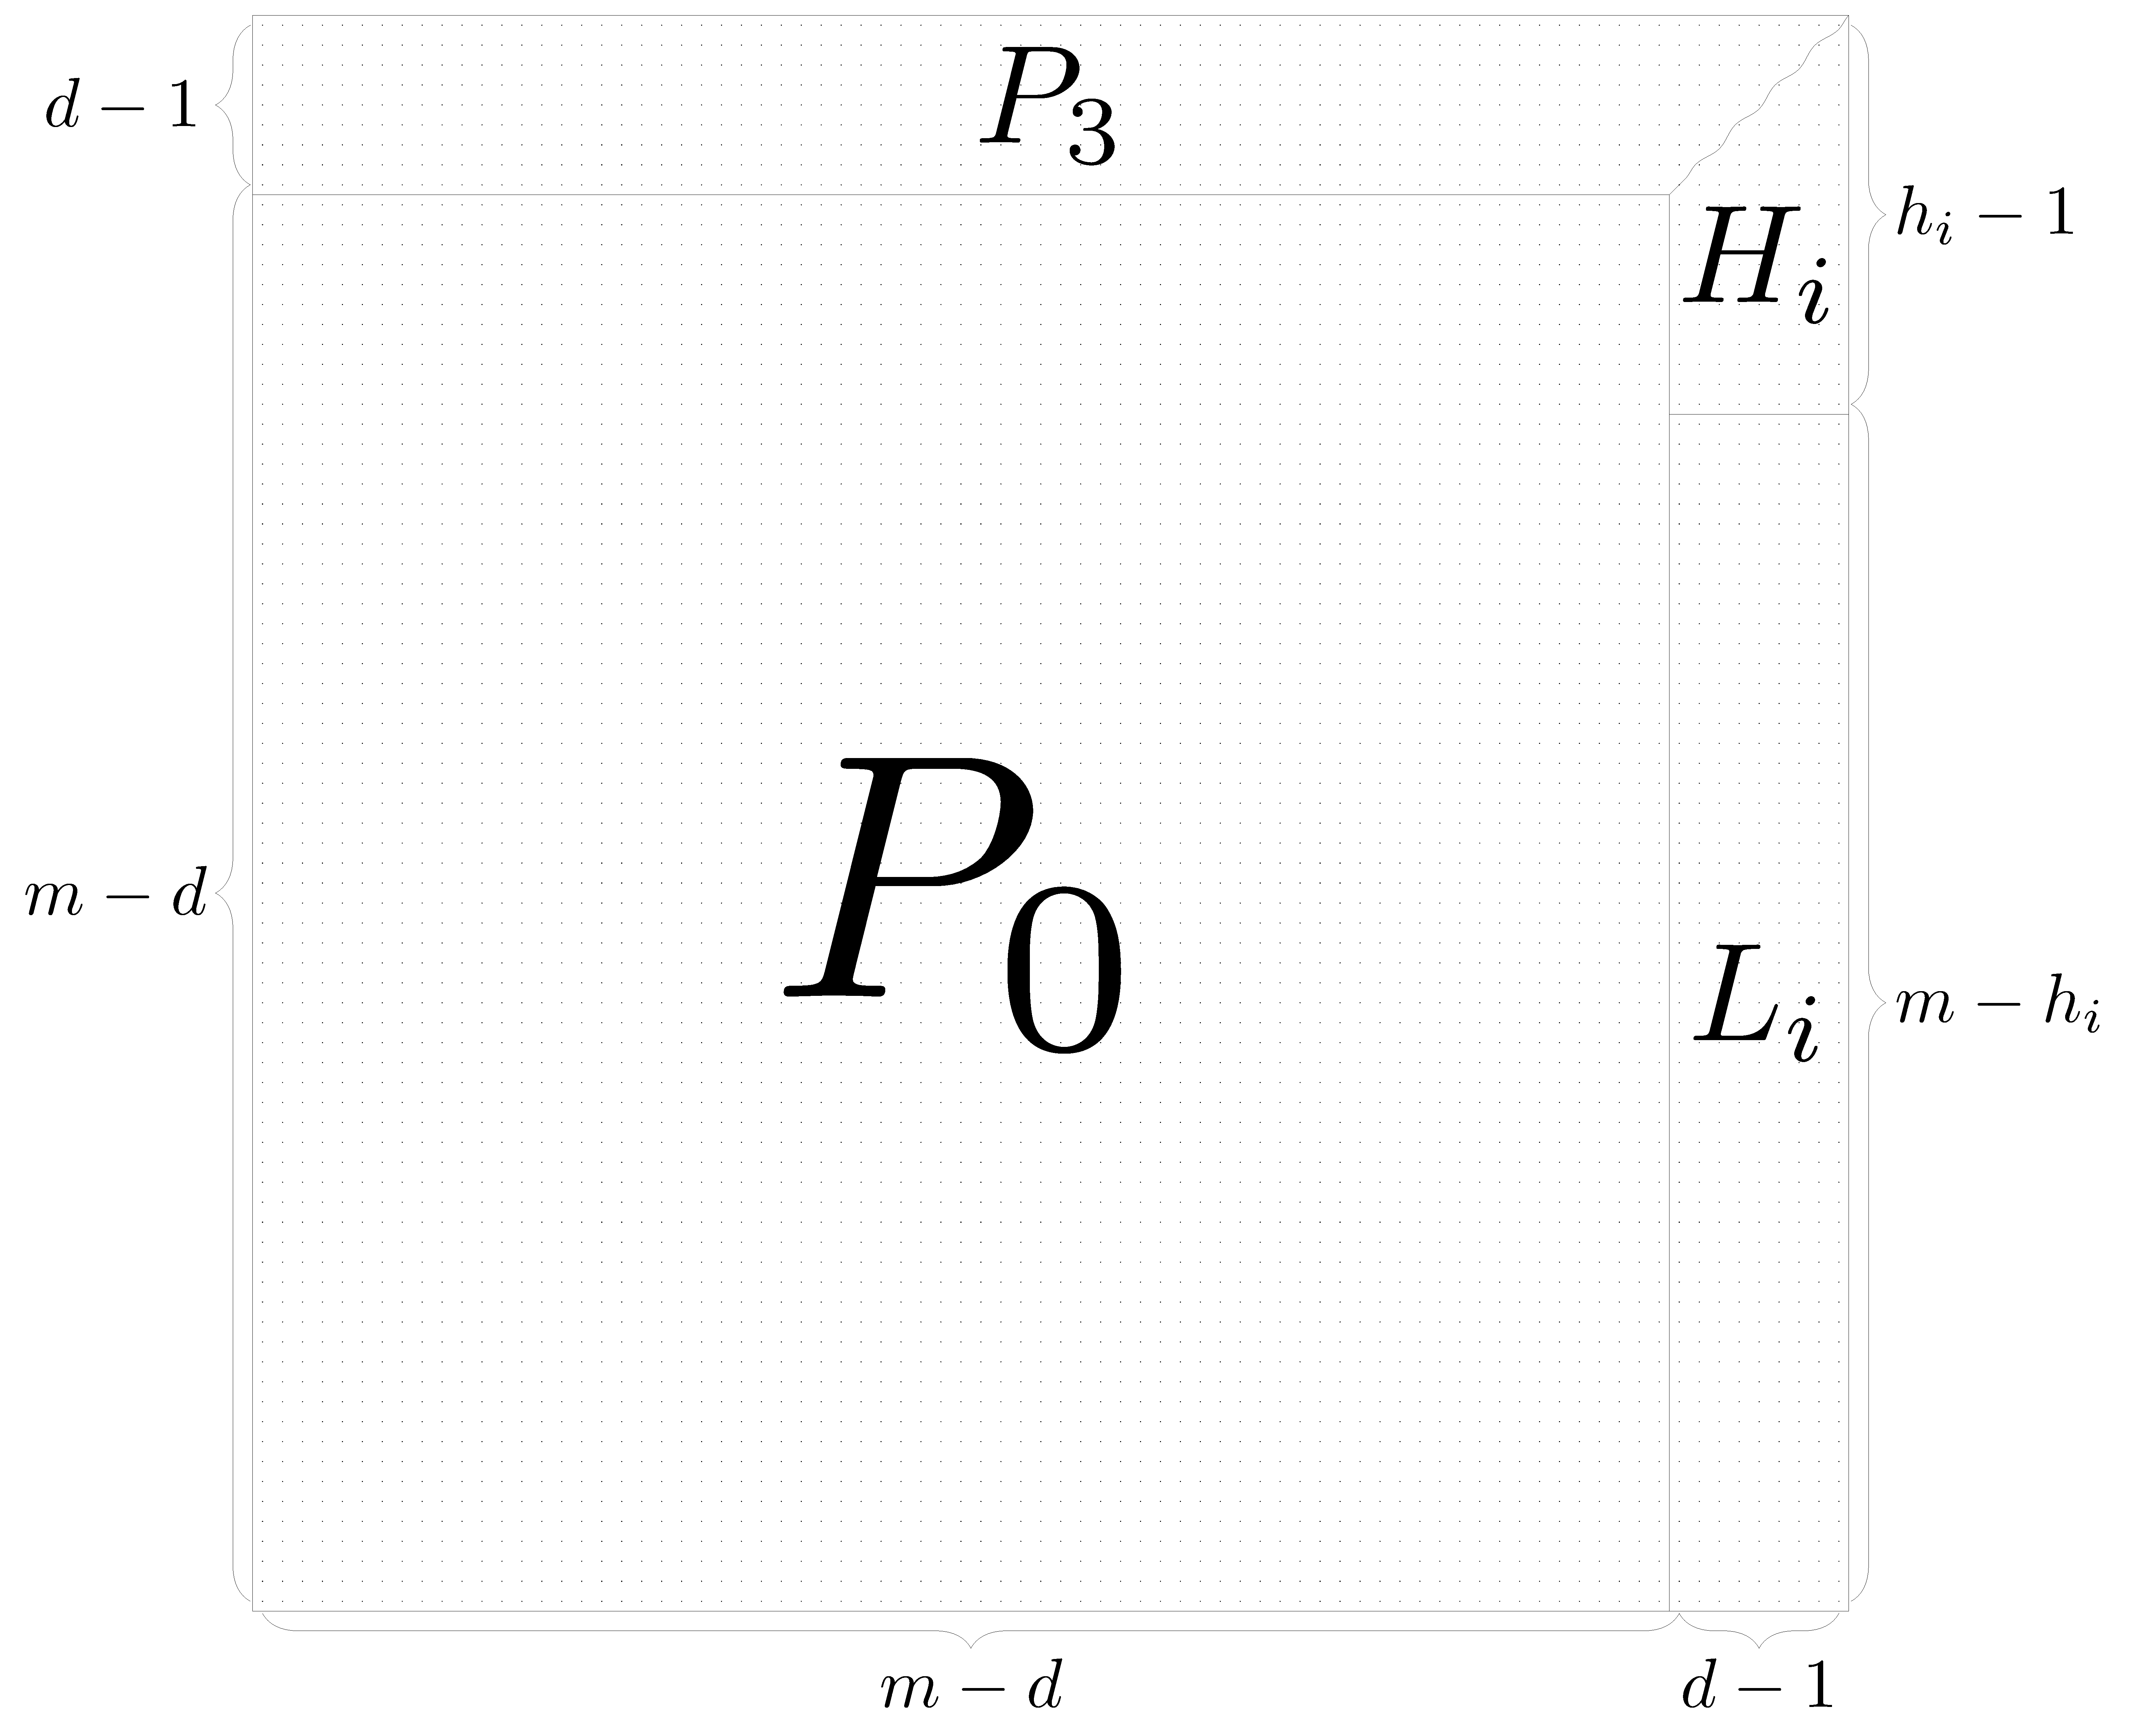
\includegraphics[width=0.8\textwidth]{drawings/pattern_restriction}
	\end{center}
	\caption{Pattern partitioning.}
	\label{figure:pattern_restriction}
\end{figure}

For each $i \in [\ell]$ we find $h_i \in \Z^+$, which we define as the minimal number such that $(\x{v}, \y{u} + h_i) \not \in \Ta$ for every $u, v \in V_i$.
For better understanding, $h_i$ is an upper bound for the height of $V_i$.

The construction is illustrated in \Cref{figure:periphery_decomposition}.
The points in the gray area are outside of the active text.
The remaining ones are in the active text, where the red and green represent $\d{S_1}$, and the green belong to some fixed $V_i$.

\begin{lemma}\label{sum_of_h}
	The sum of all $h_i$ is $\O(m)$.
	\begin{proof}
		Since for $\ell < 2$ the proof is trivial, we assume $\ell \ge 2$.
		For every $i \in [\ell]$ (since $h_i$ is minimal) there exists a pair of points $u_i, v_i \in V_i$ such that $(\x{v_i}, \y{u_i} + h_i - 1) \in \Ta$.
		It can be shown that for all $i \ge 2$ we have
		\[ h_{i} \le \y{u_{i - 2}} - \y{u_{i}} + d,\]
		since if that was not the case for some $i$, then the points $u_{i - 2}$ and $(\x{v_{i}}, \y{u_{i}} + h_{i} - 1)$ would contradict \Cref{border_lemma}.
		We can conclude that
		\[
			\sum_{i = 0}^{\ell - 1} h_i
			\le h_0 + h_1 + \sum_{i = 2}^{\ell - 1} (\y{u_{i - 2}} - \y{u_i} + d)
			= h_0 + h_1 + \y{u_0} + \y{u_1} - \y{u_{\ell - 2}} - \y{u_{\ell - 1}} + (\ell - 2)d 
			= \O(m).
		\]
	\end{proof}
\end{lemma}

\begin{observation}\label{area_bound}
	By the above lemma $|\d{S_1}| = \O(md)$ and by extension $|\d{S}| = \O(md)$.
\end{observation}

For every $i \in [\ell]$ we construct the string $L_i$ as the restriction of $P_2$ to $[m] \times [m - h_i] \cap \d{P_2}$
and the string $H_i$ as the restriction of $P_2$ to $\d{P_2} \setminus \d{L_i}$.
The construction is illustrated in \Cref{figure:pattern_restriction}.
Since $L_i$ and $H_i$ partition $P_2$, we have
\[ \Ham(P_2 + q, S_1) = \sum_{i = 0}^{\ell - 1} \Ham(P_2 + q, V_i) = \sum_{i = 0}^{\ell - 1} \Ham(L_i + q, V_i) + \sum_{i = 0}^{\ell - 1} \Ham(H_i + q, V_i). \]

\begin{lemma}\label{pattern_height_reduction}
	$\d{L_i + q} \cap \d{V_i} = \emptyset$ for every $q \in Q$ and $i \in [\ell]$.
	\begin{proof}
		Let us assume the contrary.
		Select any $q \in Q$ and $i \in [\ell]$, such that $\d{L_i + q} \cap \d{V_i}$ 
		contains some point $u$ and consider the point $v = (\x{u}, \y{u} + h_i)$.
		Since $u \in [m] \times [m - h_i] + q$, we have $v \in [m]^2 + q \subseteq \d{\Ta}$, thus $v \in \Ta$, which contradicts the definition of $h_i$.
	\end{proof}
\end{lemma}

By \Cref{pattern_height_reduction}, for every $q \in Q$ we have $\sum_{i = 0}^{\ell - 1} \Ham(L_i + q, V_i) = 0$, thus our result is equal to $\sum_{i = 0}^{\ell - 1} \Ham(H_i + q, V_i)$.
We run the algorithm from \Cref{general_fft} for every pair of $H_i$ and $V_i$ and, since both $H_i$ and $V_i$ have widths not greater than $d$ and heights not greater than $h_i$, we obtain the total complexity of $\tO(\sum_{i = 0}^{\ell - 1} (|\Sigma| + 1)dh_i)$, 
which, by \Cref{sum_of_h}, is $\tO(m^2 + md|\Sigma|)$.


% PHI PSI FINDER
\subsection{Period acquisition} \label{get_periods_proof}

This section serves as the proof of the theorem, which we used to obtain the periods $\phi$ and $\psi$:

\GetPeriods

We start by finding the closest pair of points in $U$.
Specifically, we select any pair of different points $s, t \in U$, which minimizes $|t - s|$. 
Such pair can be obtained in $\tO(|U|)$ operations, for example with a sweep line method.
We construct $w = t - s$.

We define a partial order $\le_{w}$ on $\Z^2$, where we have $u \le_w u$ for every $u \in \Z^2$ and $v \le_w u$ for some pair of different points $u, v \in \Z^2$, when at least one condition holds for $\delta = u - v$:
\begin{enumerate}[a)]
	\item $w$ and $\delta$ belong to the same quadrant, \label{quadrant_condition}
	\item $\alpha \in (-\pi / 6, \pi / 6)$, where $\alpha$ is the angle between $w$ and $\delta$. \label{angle_condition}
\end{enumerate}
Consider a vector $\rho$, where
\begin{enumerate}[$1^\circ$]
	\item if $w \in \Q_1$, then $\rho = (+\sqrt{2} / 2, +\sqrt{2} / 2)$,
	\item if $w \in \Q_2$, then $\rho = (-\sqrt{2} / 2, +\sqrt{2} / 2)$,
	\item if $w \in \Q_3$, then $\rho = (-\sqrt{2} / 2, -\sqrt{2} / 2)$,
	\item if $w \in \Q_4$, then $\rho = (+\sqrt{2} / 2, -\sqrt{2} / 2)$.
\end{enumerate}
Observe that the condition (\ref{quadrant_condition}) is equivalent to
\begin{enumerate}[a')]
	\item $\alpha \in [-\pi / 4, \pi / 4)$, where $\alpha$ is the angle between $\rho$ and $\delta$.
\end{enumerate}
Let $\beta$ be the angle between $\rho$ and $w$. Similarly, the condition (\ref{angle_condition}) is equivalent to
\begin{enumerate}[b')]
	\item $\alpha \in (\beta - \pi / 6, \beta + \pi / 6)$, where $\alpha$ is the angle between $\rho$ and $\delta$. 
\end{enumerate}
Let $R = [-\pi / 4, \pi / 4) \cup (\beta - \pi / 6, \beta + \pi / 6)$. 
We can see that the conditions (\ref{quadrant_condition}) and (\ref{angle_condition}) are thus equivalent to a single condition:
\begin{enumerate}[A)]
	\item $\alpha \in R$, where $\alpha$ is the angle between $\rho$ and $\delta$. \label{joint_condition}
\end{enumerate}
Observe that $R \subseteq (-5 \pi / 12, 5 \pi / 12)$ since $\beta \in [-\frac{\pi}{4}, \frac{\pi}{4})$.
Thus, the vectors $\delta$, which satisfy (\ref{joint_condition}), belong to a single half-plane and they satisfy $\delta \cdot \rho > \cos(5\pi / 12)|\delta||\rho| > |\delta| / 4$.
Also, since $r$ is a contiguous range of angles, for every $\delta_1$ and $\delta_2$ satisfying the condition, $\delta_1 + \delta_2$ also satisfies it.
Thus, we can prove that for every $u_1, u_2, u_3 \in \Z^2$, such that $u_1 \le_w u_2$ and $u_2 \le_w u_3$, we have $u_1 \le_w u_3$ (meaning the relation is transitive).
If $u_1 = u_2$ or $u_2 = u_3$, the proof is trivial.
If not, observe that $\delta_1 = u_2 - u_1$ and $\delta_2 = u_3 - u_1$ satisfy the condition, 
thus it also holds for $u_3 - u_1 = \delta_1 + \delta_2$.
It is also easy to prove that $\le_w$ is asymmetric.

Under the partial order $\le_w$, we find the longest chain $C$ and the longest antichain $A$ using dynamic programming.
With an appropriate data structure we can do it in $\tO(|U|)$ operations, by using a method resembling LIS calculation.

\begin{lemma}\label{C_ineq}
	$(|C| - 1) |w| < 6\ell$. 
	\begin{proof}
		Let $f = |C| - 1$ and
		let $c_0, \dots, c_{f}$ denote the points in $C$, ordered so that $c_i \le_w c_{i + 1}$ for every $i \in [f]$.
		Consider the sequence $\delta_0, \dots, \delta_{f - 1}$, where $\delta_i = c_{i + 1} - c_i$ for every $i \in [f]$.
		By definition of $w$, we have $|\delta_i| \ge |w|$,
		and since $\delta_i \cdot \rho > |\delta_i| / 4$, we get
		$\delta_i \cdot \rho > |w| / 4$ for every $i \in [f]$.
		We have
		\[ \sum_{i = 0}^{f - 1} \delta_i = c_f - c_0,\]
		and thus
		\[ f|w| / 4 < \sum_{i = 0}^{f - 1} \delta_i \cdot \rho = (c_f - c_0) \cdot \rho \le \ell \sqrt{2}, \]
		which gives us $(|C| - 1)|w| < 4\ell \sqrt{2} < 6\ell$.
	\end{proof}
\end{lemma}

\begin{lemma}[Dilworth's theorem]\label{dilworth}
	$|U| \le |C| |A|$.
\end{lemma}

We know that $|C| \ge 2$, since there exists a chain containing $s$ and $t$.
By \cref{C_ineq}, we have
\[ |C||w| / 2 \le (|C| - 1)|w| < 6\ell, \]
and thus
\[ |C| \le |C||w| < 12\ell. \]
By the assumption $|U| \ge 12\ell$ and \Cref{dilworth}
\[12 \ell < |U| \le |C| |A| < 12\ell|A|,\]
thus $|A| > 1$, which means $|A| \ge 2$.
We select any pair of different vectors $s', t' \in A$, which minimizes $|t' - s'|$ and construct $w' = t' - s'$.
We will now show that $|w||w'| = \O(\ell^2 / |U|)$.

\begin{lemma}\label{A_ineq}
	$(|A| - 1) |w'| \le 2\ell$. 
	\begin{proof}
		Recall that $(-\pi / 4, \pi / 4) \subseteq r$.
		Define a range of angles $R' = [\pi / 4, 3\pi / 4]$.
		Consider any $u, v \in \Z^2$, such that $u \not \le_w v$ and $v \not \le_w u$.
		It can be shown that the angle between $\rho$ and $\delta$ is in $R'$ for some $\delta \in \set{u - v, v - u}$.
		Thus $|(u - v) \times \rho| \ge \sin(\pi / 4) |u - v||\rho| = |u - v|\sqrt{2} / 2$.
		
		Let $f = |A| - 1$ and let $a_0, \dots, a_{f}$ be the points in $A$ ordered such that $a_i \times \rho \le a_{i + 1} \times \rho$ for every $i \in [f]$.
		Consider the sequence $\delta_0, \dots, \delta_{f - 1}$, where $\delta_i = a_{i + 1} - a_i$ for every $i \in [f]$.
		By definition of $w'$, we have $|\delta_i| \le |w'|$ and since $|\delta_i \times \rho| \ge |\delta_i|\sqrt{2} / 2$, we get $\delta_i \times \rho = |\delta_i \times \rho| \ge |w| \sqrt{2} / 2$ for every $i \in [f]$.
		We have
		\[ \sum_{i = 0}^{f - 1} \delta_i = a_f - a_0,\]
		and thus
		\[ f|w'| \sqrt{2}/2 \le \sum_{i = 0}^{f - 1} \delta_i \times \rho = (c_f - c_0) \times \rho \le \ell \sqrt{2}, \]
		which gives us $(|A| - 1)|w| \le 2\ell$.
	\end{proof}
\end{lemma}

By \Cref{A_ineq}, and since $|A| \ge 2$, we have
\[|A||w'| \le 2(|A| - 1) |w'| \le 4\ell.\]
Recall that $|C||w| < 12\ell$ and $|U| \le |C| |A|$. We can multiply the inequalities and obtain
\[ |U||w||w'| \le |C||A||w||w'| < 48 \ell^2,\]
which finally gives us
\[|w||w'| < \frac{48\ell^2}{|U|} = \O(\ell^2 / |U|). \]
It can be easily shown that $w, w'$ satisfy the remaining conditions by the definition of $\le_w$.


% SUBPARQUET CONVOLUTION
\newcommand{\W}{\mathcal{W}}
\subsection{Subparquet convolution} \label{subparquet_convolution_proof}

Throughout this section we will denote $D = \set{u : u \in \L, \h{u} \ge 0, \s{u} \ge 0}$, where $\L$ is the set defined in \Cref{lattice_congruency}.
We start by introducing some auxiliary tools, which we later use in the proof of \Cref{sparse_algo}.

\begin{lemma}\label{primitive_conv}
	Given a set of subparquets $\V$ and a set of points $Q$, we can calculate
	\[ \sum_{V \in \V} |(D + q) \cap V| \]
	for every $q \in Q$ in total time $\tO(n^2 + |Q| + |\V|)$, assuming that every $V \in \V$ consists of vectors of length $\O(n)$.
	\begin{proof}
		For every $u \in \Z^2$ let us define $\score(u) = |\set{V : V \in \V, u \in V}|$. Observe that
		\[ \sum_{V \in \V} |(D + q) \cap V| = \sum_{u \in D + q} \score(u). \]
		We start by explicitly calculating the scores.
		We find the maximum length of a vector that some $V \in \V$ contains, which we denote $\ell$.
		We construct the set $U \subseteq \Z^2$ of all vectors of length at most $\ell$.
		By the assumption, we have $\ell = \O(n)$, and thus $|U| = \O(\ell ^ 2) = \O(n ^ 2)$.
		Since all the scores are zero for points outside of $U$, will only calculate them for $u \in U$.
		
		We find the set $\Gamma$ introduced in \Cref{lattice_base} and for every $\gamma \in \Gamma$ we construct $U_\gamma = U \cap (\L + \gamma)$.
		Consider any $u \in U_\gamma$ for some fixed $\gamma \in \Gamma$ and any $V \in \V$.
		Observe that if $V \not \equiv \gamma$, then $u \not \in V$ and thus $V$ does not contribute to $\score(u)$.
		If $V \equiv \gamma$, then we can find a parquet $W$ such that $V = W \cap (\L + \gamma)$ and we have
		$u \in V \Leftrightarrow u \in W \cap (\L + \gamma) \Leftrightarrow u \in W$.
		Thus, if we denote $\W_\gamma$ as the set of parquets $W$ obtained for every $V \in \V$ such that $V \equiv \gamma$, then $\score(u)$ for $u \in U_\gamma$ is the number of parquets $W \in \W_\gamma$ such that $u \in W$.
		We calculate $\score(u)$ for every $u \in U_\gamma$ by sweeping $U_\gamma$ and $\W_\gamma$ in time $\tO(|U_\gamma| + |\W_\gamma|)$.
		We do it independently for every $\gamma \in \Gamma$, performing $\tO(|U| + |\V|) = \tO(n^2 + |\V|)$ operations in total.

		Now consider a query vector $q \in Q$.
		Let $\gamma \in \Gamma$ be such that $q \equiv \gamma$.
		We have already shown that the sum of scores for $u \in D + q$ is equal to the sum of scores for $u \in (D + q) \cap U$.
		Since $(D + q) \cap U = (D + q) \cap U_\gamma$, we see that the result is the sum of scores for such $u \in U_\gamma$, for which $\h{u} \ge \h{q}$ and $\s{u} \ge \s{q}$.
		If we denote $Q_\gamma = Q \cap (\L + \gamma)$, we see that we can calculate the results for all $q \in Q_\gamma$ by sweeping $Q_\gamma$ and $U_\gamma$ in time $\tO(|Q_\gamma| + |U_\gamma|)$.
		We do it independently for every $\gamma \in \Gamma$, performing $\tO(|Q| + |U|) = \tO(n^2 + |Q|)$ operations in total.
	\end{proof}
\end{lemma}

\begin{lemma}\label{primitive}
	For any simple subparquet $U$ we can find $w_0, \dots, w_3 \in \Z^2$, such that
	\[ |U \cap X| = \sum_{j = 0}^3 (-1)^j |(D + w_j) \cap X|\]
	for every $X \subseteq \Z^2$.
	If $U$ consists of vectors of length $\O(n)$, then $w_0, \dots, w_3$ are of length $\O(n)$.
	\begin{proof}
		Let \eq{
			\phi_0 = \min\set{{\h{u} : u \in U}}, \quad 
			\phi_1 = \max\set{{\h{u} : u \in U}},\\
			\psi_0 = \min\set{{\s{u} : u \in U}}, \quad
			\psi_1 = \max\set{{\s{u} : u \in U}}.
		}
		Note that these values can be extracted from the signature.
		Since $U$ is a parquet, there exist unique points $u_0, \dots, u_3 \in U$, such that
		\begin{itemize}
			\item $\h{u_0} = \phi_0$ and $\s{u_0} = \psi_0$,
			\item $\h{u_1} = \phi_1$ and $\s{u_1} = \psi_0$,
			\item $\h{u_2} = \phi_1$ and $\s{u_2} = \psi_1$,
			\item $\h{u_3} = \phi_0$ and $\s{u_3} = \psi_1$.
		\end{itemize}
		We construct \eq{
			w_0 = u_0, \quad 
			w_1 = u_1 + \psi, \quad
			w_2 = u_2 + \phi + \psi, \quad
			w_3 = u_3 + \phi.
		}
		It can be proven that the condition is satisfied.
	\end{proof}
\end{lemma}

\begin{theorem}\label{subparquet_convolution}
	For a given list of signatures of simple subparquets $U_0, \dots, U_{\ell - 1}$, list of signatures of subparquets $V_0, \dots, V_{\ell - 1}$ and a set of vectors $Q$ we can calculate
	\[ \sum_{i = 0}^{\ell - 1} |(U_i + q) \cap V_i| \]
	for every $q \in Q$ in total time $\tO(m^2 + \ell + |Q|)$, assuming that the subparquets only contain vectors of length $\O(m)$.
	\begin{proof}
		We apply \Cref{primitive} to every $U_i$ and find $w_{i, 0}, \dots, w_{i, 3}$, so that we have
		\eq{
			\sum_{i = 0}^{\ell - 1}|(U_i + q) \cap V_i| 
			= \sum_{i = 0}^{\ell - 1}|U_i \cap (V_i - q)| 
			= \sum_{i = 0}^{\ell - 1} \sum_{j = 0}^3 (-1)^j |(D + w_{i, j}) \cap (V_i - q)| = \\
			= \sum_{j = 0}^3 (-1)^j \sum_{i = 0}^{\ell - 1} |(D + q) \cap (V_i - w_{i, j})|.
		}
		By \Cref{primitive_conv} we can independently calculate the values $\sum_{i = 0}^{\ell - 1} |(D + q) \cap (V_i - w_{i, j})|$ for every $j$ by running the algorithm for $\V_j = \set{V_i - w_{i, j} : i \in [\ell]}$ and $Q$.
	\end{proof}
\end{theorem}

\SparseAlgo
\begin{proof}
	Let $U = \bigcup_{S \in \S} \d{S}$. Observe that
	\[ \sum_{S \in \S} \Ham(P + q, S) = |\d{P + q} \cap U| - \sum_{S \in \S}\sum_{V \in \V_{\getchar{S}}} |\d{V + q} \cap \d{S}|.\]
	We can calculate $|\d{P + q} \cap U|$ for every $q \in Q$ with a single instance of FFT (see \Cref{sigman2d}) or by using prefix sums in time $\tO(m^2)$.
	To calculate the values
	\[ \sum_{S \in \S}\sum_{V \in \V_{\getchar{S}}} |\d{V + q} \cap \d{S}| \]
	we use the algorithm from \Cref{subparquet_convolution} (where $\ell = \sum_{S \in \S} |\V_{\getchar{S}}|$).
\end{proof}


% PARQUET DECOMPOSITION
\subsection{Periodic parquet partitioning} \label{parquet_decomposition_proof}
In this section we explore the properties of periodic (sub-)parquet strings (recall Definitions \ref{parquet_definition}, \ref{subparquet_definition}, \ref{parquet_string_definition}).
Specifically, we introduce some methods of partitioning them into monochromatic strings, which we utilize when decomposing both the pattern and the active text.

\begin{definition}[Lattice graph]
	For a set $U \subseteq \Z^2$ we define its \textbf{lattice graph} $(U, \Edges(U))$, where
	\[ \Edges(U) = \bigset{\set{u, u + \delta} : \delta \in \set{\phi, \psi}, u \in U, u + \delta \in U},\] 
	so every vector is connected with its translations by $\phi, \psi, -\phi, -\psi$, which are contained in $U$.
\end{definition}


\begin{lemma}\label{lattice_graph_connectivity}
	If $U$ is a spacious subparquet, then $(U, \Edges(U))$ is connected.
	\begin{proof}
		Assume the contrary.
		Consider any pair of points $u, v \in U$, such that
		\begin{itemize}
			\item $u$ and $v$ belong to different connected components,
			\item if we let $s, t \in \Z$ be such that $v = u + s \phi + t \psi$, then $|s| + |t|$ is minimized.
		\end{itemize}
		Let us assume that for such $u$ and $v = u + s \phi + t \psi$ we have $s \ge 0$, since in the other case they can be swapped.
		We now show that there exists a point $w \in U$, such that $\set{u, w} \in \Edges(U)$ and if we let $s', t' \in \Z$ be such that $v = w + s'\phi + t'\psi$, then $|s'| + |t'| < |s| + |t|$, which contradicts the minimality of $|s| + |t|$. 
	
		Let $x_0, x_1, y_0, y_1, \phi_0, \phi_1, \psi_0, \psi_1 \in \Z$ be such that
		\begin{itemize}
			\item $ U = [x_0, x_1] \times [y_0, y_1] \cap \set{w : w \in \Z^2, \h{w} \in [\phi_0, \phi_1], \s{w} \in [\psi_0, \psi_1], w \equiv u}$,
			\item $x_1 - x_0 + 1 \ge |\x{\phi}| + |\x{\psi}|$ and $y_1 - y_0 + 1 \ge |\y{\phi}| + |\y{\psi}|$.
		\end{itemize}
		They exist by definition of a spacious subparquet.
		Recall that $\x{\phi} \ge 0$, $\y{\phi} \le 0$, $\x{\psi} \ge 0$, $\y{\psi} \ge 0$.
		We have the following cases:
		\begin{enumerate}[$1^\circ$]
			\item If $s = 0$ and $t > 0$, then $w = u + \psi$. Observe that
				\eq{
					\x{u} \le \x{w} \le \x{v}, \quad \y{u} \le \y{w} \le \y{v}, \quad \h{u} \le \h{w} \le \h{v}, \quad \s{w} = \s{u},
				}
				and since $w \equiv u$, we get $w \in U$.
			\item If $s = 0$ and $t < 0$, then $w = u - \psi$ and we can similarly show that $w \in U$, since
				\[\x{v} \le \x{w} \le \x{u}, \quad \y{v} \le \y{w} \le \y{u}, \quad \h{v} \le \h{w} \le \h{u}, \quad \s{w} = \s{u}.\]
			\item If $s > 0$ and $t = 0$, then $w = u + \phi$ and we get $w \in U$, since
				\[\x{u} \le \x{w} \le \x{v}, \quad \y{v} \le \y{w} \le \y{u}, \quad \h{v} = \h{u}, \quad \s{v} \le \s{w} \le \s{u}.\]
			\item If $s > 0$ and $t > 0$, consider the point $w' = u + \phi$. \label{case_pos}
				We have \eq{
					\x{u} \le \x{w'} \le \x{v}, \quad \h{w'} = \h{u}, \quad \s{v} \le \s{w'} \le \s{u}.
				}
				If $w' \in U$, then $w = w'$.
				If $w' \not \in U$, then since all other requirements are satisfied, we must have $\y{w'} \not \in [y_0, y_1]$.
				Since $\y{w'} = \y{u} + \y{\phi} \le \y{u}$, we have $\y{u} + \y{\phi} \le y_0 - 1$, and
				considering $y_1 - y_0 + 1 \ge |\y{\phi}| + |\y{\psi}|$, we get $y_1 \ge \y{u} + \y{\psi}$.
				Now let $w = u + \psi$.
				We have \eq{
					\x{u} \le \x{w} \le \x{v}, \quad \y{u} \le \y{w} = \y{u} + \y{\psi} \le y_1, \quad \h{u} \le \h{w} \le \h{v}, \quad \s{w} = \s{u},
				}
				thus $w \in U$.
			\item If $s > 0$ and $t < 0$, consider $w' = u + \phi$.
				We have \eq{
					\y{v} \le \y{w'} \le \y{u}, \quad \h{w'} = \h{u}, \quad \s{v} \le \s{w'} \le \s{u}.
				}
				If $w' \in U$, then $w = w'$.
				Otherwise we can (similarly to $\ref{case_pos}^\circ$) show that $w = u - \psi \in U$, by the fact that $x_1 - x_0 + 1 \ge |\x{\phi}| + |\x{\psi}|$. \qedhere
		\end{enumerate}
	\end{proof}
\end{lemma}


\begin{figure}[!t]
	\begin{center}
		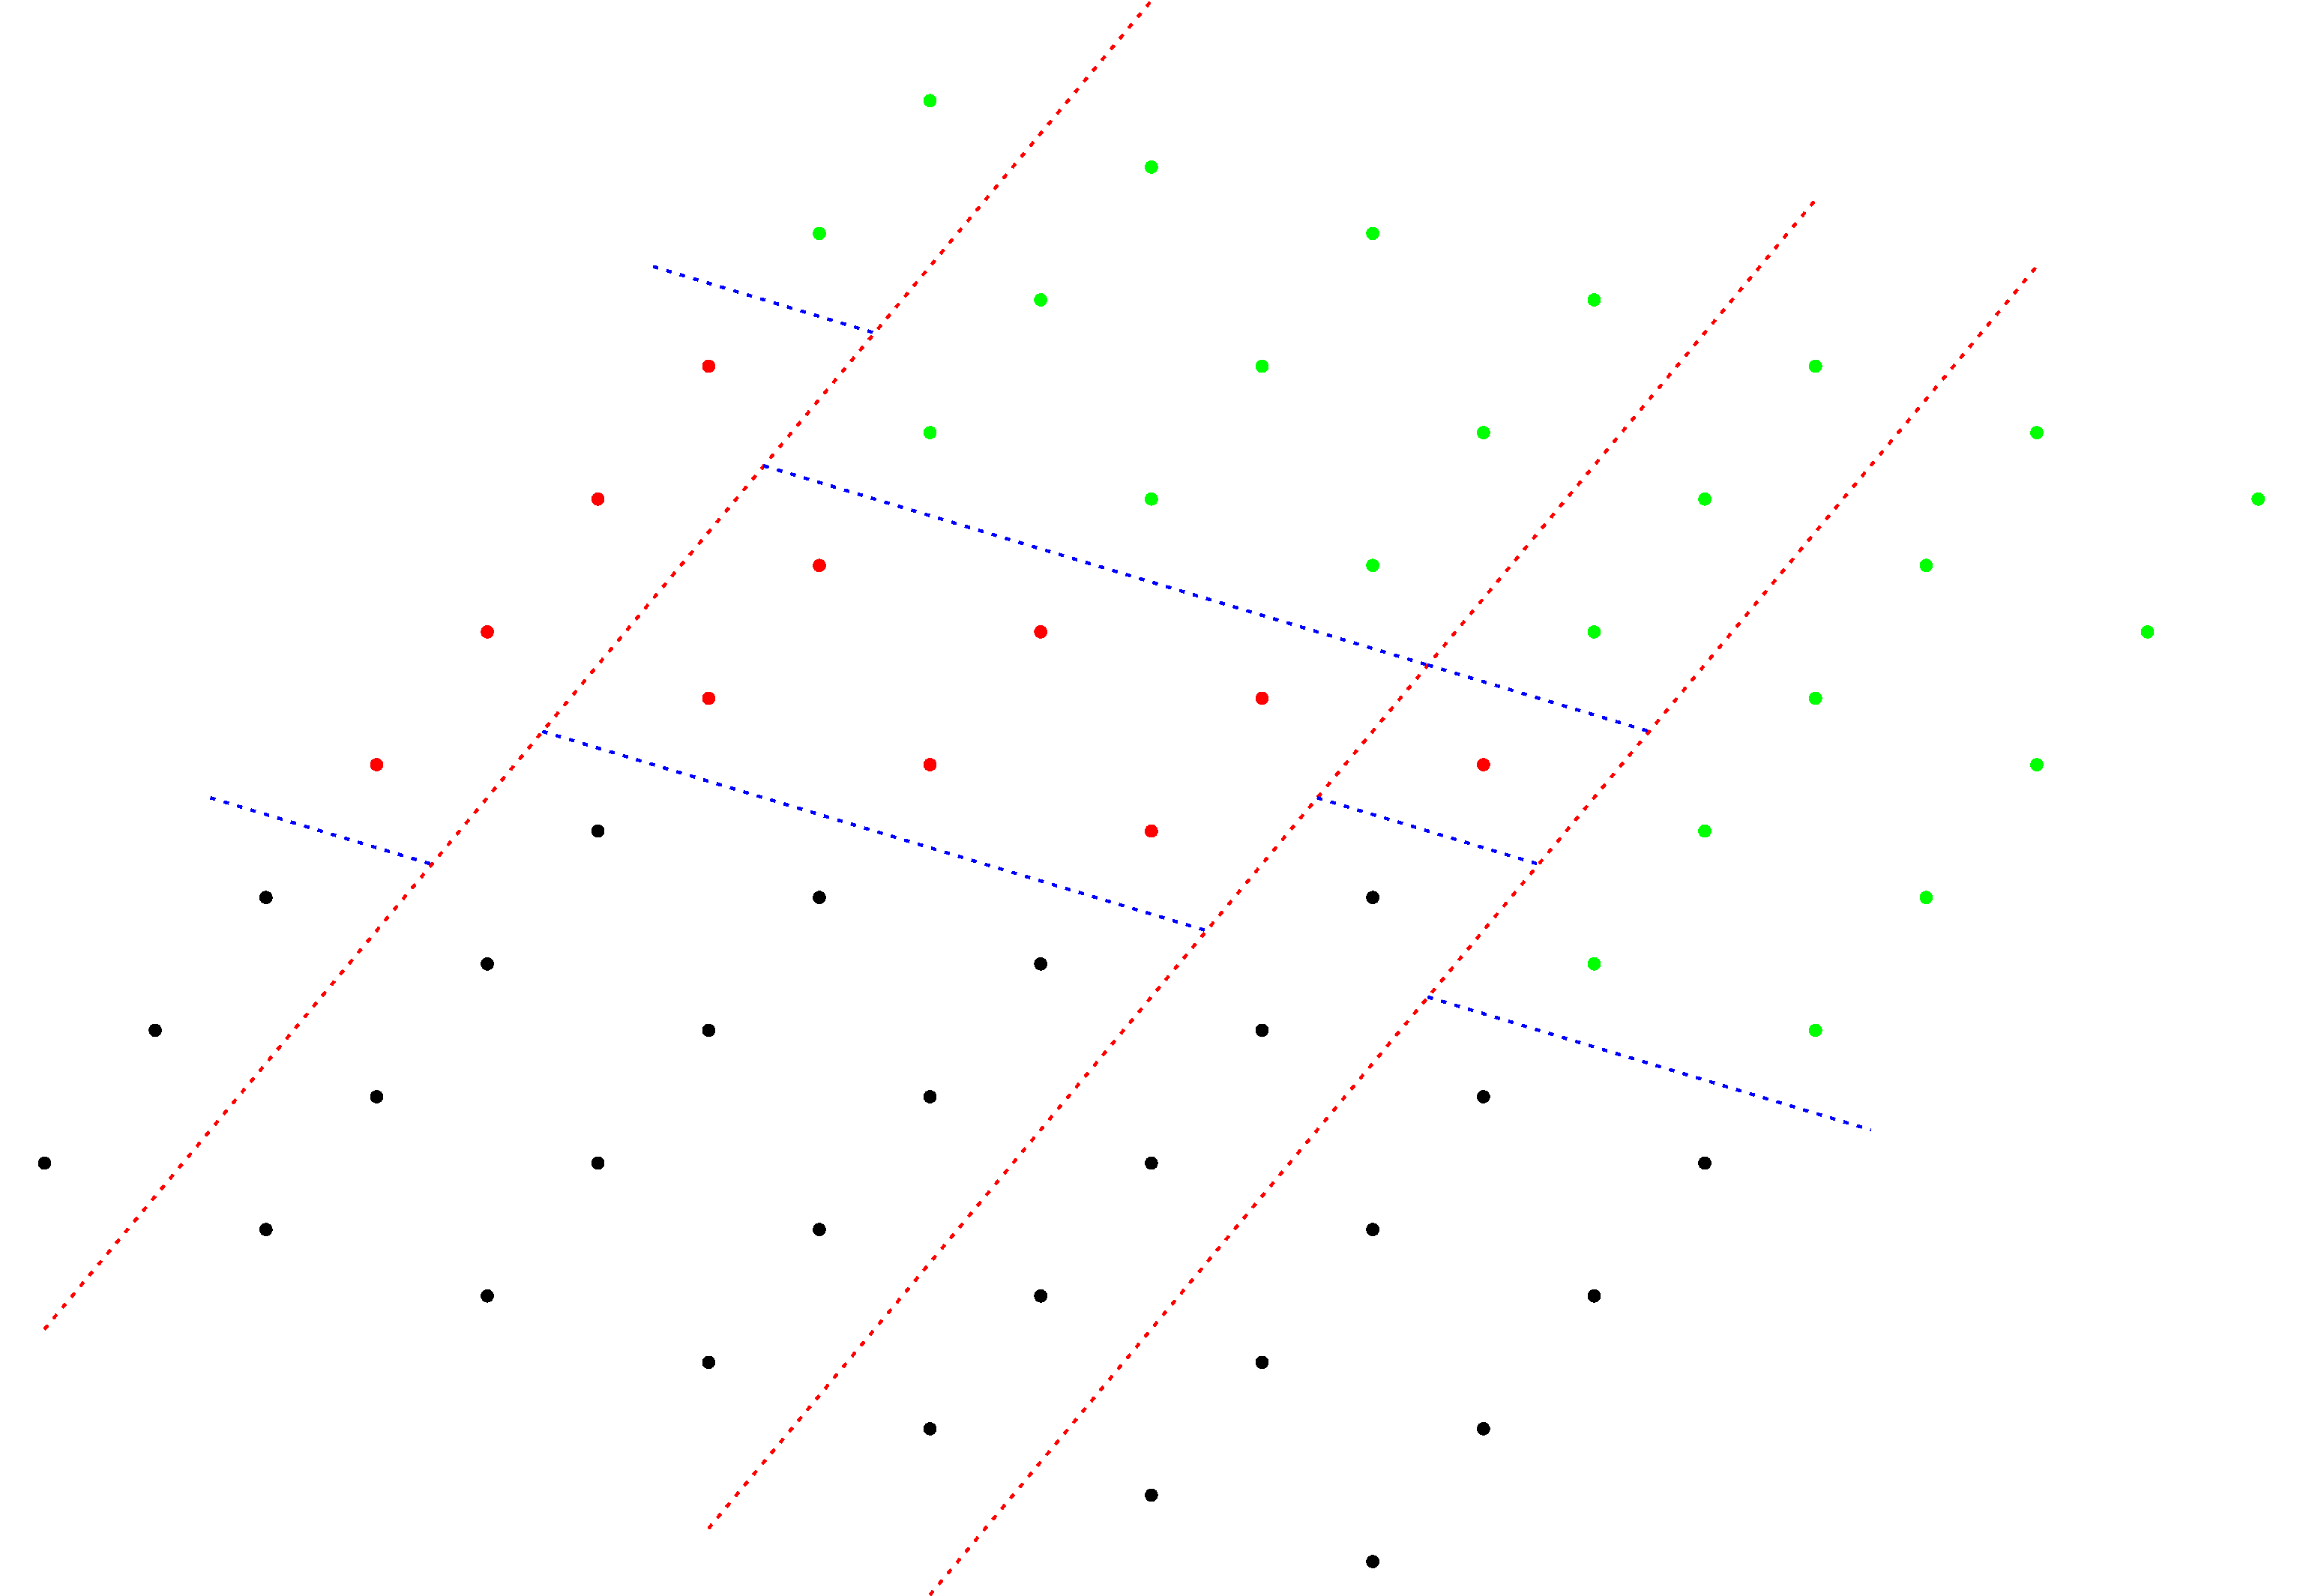
\includegraphics[width=0.8\textwidth]{drawings/parquet_decomposition}
	\end{center}
	\caption{The partitioning of a simple subparquet string into monochromatic simple subparquet strings. Different colors represent different characters assigned to a point.}
	\label{figure:parquet_decomposition}
\end{figure}


\begin{lemma}\label{monochromacy_condition}
	A spacious subparquet string $S$ is monochromatic if and only if
	\[\Ham(S + \phi, S) + \Ham(S + \psi, S) = 0.\]
	\begin{proof}
		If $S$ is monochromatic, then clearly $\Ham(S + \phi, S) + \Ham(S + \psi, S) = 0$.
		Assume the contrary for the other implication.
		Let $u, v \in S$ be such that $S(u) \neq S(v)$.
		Since $\d{S}$ is a spacious subparquet, the graph $(\d{S}, \Edges(\d{S})$ is connected (by \Cref{lattice_graph_connectivity}) and there must exist a path between $u$ and $v$.
		On that path there must exist a pair of neighbors $w, w'$, such that $S(w) \neq S(w')$ and $w' = w + \delta$ for some $\delta \in \set{\phi, \psi}$.
		If $\delta = \phi$, then $\Ham(S + \phi, S) \ge 1$ and if $\delta = \psi$, then $\Ham(S + \psi, S) \ge 1$ and we get a contradiction.
	\end{proof}
\end{lemma}


\begin{lemma}\label{cut_partitioning}
	A spacious subparquet string $S$ can be partitioned in time $\tO(|\d{S}| + 1)$ into both the following sets of strings (we have two options):
	\begin{enumerate}[a)]
		\item a set of $\O(\Ham(S + \phi, S) + 1)$ strings $\U$, such that $\Ham(U + \phi, U) = 0$ for each $U \in \U$ and \label{partition_a}
		\item a set of $\O(\Ham(S + \psi, S) + 1)$ strings $\V$, such that $\Ham(V + \psi, V) = 0$ for each $V \in \V$. \label{partition_b}
	\end{enumerate}
	All the obtained strings are spacious and if $S$ is simple, they are simple.
	\begin{proof}
		Let us consider option (\ref{partition_a}). We construct the set
		\[ A = \set{\s{u} : u \in S, u + \phi \in S, S(u) \neq S(u + \phi)} \cup \set{-\infty, +\infty}\]
		and then sort its elements increasingly, creating a sequence $a_0, \dots, a_\ell$.
		Note that $\ell \le \Ham(S + \phi, S) + 2$.
		We then construct the strings $S_0, \dots, S_{\ell - 1}$, where $S_i$ is the restriction of $S$ to
		$\set{u : u \in S, \s{u} \in [a_i, a_{i + 1})}$ for every $i \in [\ell]$.
		Observe that $S_0, \dots, S_{\ell - 1}$ partition $S$ and that $\Ham(S_i + \phi, S_i) = 0$ for every $i \in [\ell]$.
		Also, is $S$ is spacious, then they are spacious and if $S$ is simple, then they are simple.
	
		In the case of option (\ref{partition_b}), we similarly construct
		\[ A = \set{\h{u} : u \in S, u + \psi \in S, S(u) \neq S(u + \psi)} \cup \set{-\infty, +\infty} \]
		and then sort it increasingly, creating $a_0, \dots, a_\ell$, where $\ell \le \Ham(S + \psi, S) + 2$.
		We then construct the strings $S_0, \dots, S_{\ell - 1}$, where $S_i$ is the restriction of $S$ to 
		$\set{u : u \in S, \h{u} \in (a_i, a_{i + 1}]}$.
	\end{proof}
\end{lemma}

\ParquetDecomposition
\begin{proof}
	We partition $R$ into a set of subparquet strings $\S$, such that $|\S| = \O(\min\set{m, k})$.
	Specifically, for each $\gamma \in \Gamma$ (see \Cref{lattice_base}), we construct a restriction of $R$ to $\d{R} \cap (\L + \gamma)$.
	Observe that if $R$ is spacious, then all $S \in \S$ are spacious and if $R$ is simple, then all $S \in \S$ are simple.
	We now partition each $S \in \S$ independently by using \Cref{cut_partitioning} (\ref{partition_a})
	and construct a set of subparquet strings $\S'$, such that $\S'$ partitions $R$ and $\Ham(S' + \phi, S') = 0$ for every $S' \in \S'$.
	Note that
	\[ |S'| = \sum_{S \in \S} \O(\Ham(S + \phi, S) + 1) = \O(\Ham(R + \phi, R) + |\S|) = \O(k),\]
	since $R$ has an $\O(k)$-period $\phi$.
	We now partition each $S' \in \S'$ by using \Cref{cut_partitioning} (\ref{partition_b}) and construct a set of subparquet strings $\S''$, such that $\S''$ partitions $R$ and $\Ham(S'' + \psi, S'') = 0$ for every $S'' \in \S''$.
	Again we have
	\[ |S''| = \sum_{S' \in \S'} \O(\Ham(S' + \psi, S') + 1) = \O(\Ham(R + \psi, R) + |\S'|) = \O(k),\]
	since $R$ has an $\O(k)$-period $\psi$.
	The process is illustrated in \Cref{figure:parquet_decomposition}.
	The red lines represent the partitioning done in the first phase, when constructing $\S'$, and blue in the second, when constructing $\S''$.
	By \Cref{monochromacy_condition}, the strings $S'' \in \S''$ are monochromatic.
	The total number of operations is $\tO(|\d{R}| + k)$.
\end{proof}

% TEXT DECOMPOSITION
\subsection{Active text decomposition} \label{text_decomposition_proof}

This section serves as the proof of the following major theorem:

\TextDecomposition

We will use a more geometrical approach and construct some lines and parallelograms.
For the sake of simplicity, we will consider an empty set to be a valid parallelogram.
Also, we assume that a parallelogram contains the points laying on its border and its vertices.

\begin{definition}
	For a set of points $U \subseteq \R^2$ we will denote
	\[ \X(U) = \set{\x{u} : u \in U}, \quad \Y(U) = \set{\y{u} : u \in U}.\]
\end{definition}

\newcommand{\IQ}{\mathbb{R} \setminus \mathbb{Q}}
\begin{observation}\label{line_existence}
	For any given $\ell \in \Z^+$ and $v \in \Z^2$ we can find a sequence of parallel lines $f_0, f_1, \dots, f_\ell$, where $f_i = \set{u : u \in \R^2, v \times u = c_i}$ for some $c_i \in \IQ$, such that
	\begin{itemize}
		\item $c_0 < v \times u < c_\ell$ for every $u \in [n]^2$, or namely, the set $[n]^2$ is between $f_0$ and $f_\ell$,
		\item $0 < c_{i + 1} - c_i = \O(n|v| / \ell)$ for every $i \in [\ell]$, or namely, the distance between every two consecutive lines is $\O(n / \ell)$.
	\end{itemize}
\end{observation}

We use \Cref{line_existence} with $v = \phi$ to construct the lines $h_0, \dots, h_\ell$ and with $v = \psi$ to construct the lines $s_0, \dots, s_\ell$.
For every $i, j \in [\ell + 1]$ we construct a point $w_{i, j}$ as an intersection of $h_i$ and $s_j$ (since $\phi$ and $\psi$ are not colinear, $h_i$ and $s_j$ are not parallel).
For every $i, j \in [\ell]$ we construct a parallelogram $p_{i, j}$ defined as the area between $s_i$ and $s_{i + 1}$ intersected with the area between $h_j$ and $h_{j + 1}$.
Specifically,
\[p_{i, j} = \set{u : u \in \R^2, \h{u} \in [\h{w_{i, j}}, \h{w_{i + 1, j + 1}}], \s{u} \in [\s{w_{i, j}}, \s{w_{i + 1, j + 1}}]}.\]
For better reference, the vertices of $p_{i, j}$ are $w_{i, j}, w_{i + 1, j}, w_{i + 1, j + 1}, w_{i, j + 1}$.
Observe that every $u \in [n]^2$ is contained strictly in the interior of exactly one parallelogram $p_{i, j}$.

\begin{lemma}\label{monotonicity_lemma}
	For every $i \in [\ell - 1]$ and $j \in [\ell]$ we have
	\eq{
	\min \X(p_{i, j}) < \min \X(p_{i + 1, j}), \quad
	&\min \Y(p_{i, j}) \le \min \Y(p_{i + 1, j}), \\
	\max \X(p_{i, j}) < \max \X(p_{i + 1, j}), \quad
	&\max \Y(p_{i, j}) \le \max \Y(p_{i + 1, j})
	}
	and for every $i \in [\ell]$ and $j \in [\ell - 1]$ we have
	\eq{
		\min \X(p_{i, j}) \ge \min \X(p_{i, j + 1}), \quad
		&\min \Y(p_{i, j}) < \min \Y(p_{i, j + 1}), \\
		\max \X(p_{i, j}) \ge \max \X(p_{i, j + 1}), \quad
		&\max \Y(p_{i, j}) < \max \Y(p_{i, j + 1}).
	}
	\begin{proof}
		It follows from the fact that we selected $\phi \in [0, +\infty) \times (-\infty, 0)$ and $\psi \in (0, +\infty) \times [0, +\infty)$.
		For example, to prove the first inequality, we can consider a point $u \in p_{i + 1, j}$, such that $\x{u} = \min \X(p_{i + 1, j})$
		and then construct a point $v \in p_{i, j}$, such that $v = u - t\psi$ for some $t > 0$, and thus $\min \X(p_{i, j}) \le \x{v} < \x{u} = \min \X(p_{i + 1, j})$.
		The other inequalities can be proven analogously.
	\end{proof}
\end{lemma}

\begin{restatable*}{lemma}{DistanceBoundLemma}\label{distance_bound_lemma}
	For every $i, j \in [\ell]$ and every $u, v \in \X(p_{i, j}) \times \Y(p_{i, j})$, we have $|u - v| = \O(n / \ell)$.
\end{restatable*}
\begin{proof} See \Cref{distance_bound_lemma_proof}. \end{proof}

Consider the case when $\max \X(p_{i, j}) - \min \X(p_{i, j}) \ge m / 4$ for some $i, j \in [\ell]$.
By \Cref{distance_bound_lemma}, we would have $m / 4 \le \max \X(p_{i, j}) - \min \X(p_{i, j}) = \O(n / \ell)$, and thus $\ell = \O(1)$.
In that case we can return a trivial partitioning where $F = \Ta$ and the set of monochromatic strings is empty, since $\Ta$ is $\O(m)$-peripheral.
We can use the same argument if we have $\max \Y(p_{i, j}) - \min \Y(p_{i, j}) \ge m / 4$ for some $i, j \in [\ell]$.
Thus, from now on we will assume that $\max X_{i, j} - \min X_{i, j} < m / 4$ and $\max Y_{i, j} - \min Y_{i, j} < m / 4$ for every $i, j \in [\ell]$. 

Let $z = \frac{n - 1}{2}$. 
We split the plane with two lines $x = z$ and $y = z$ into four quarters:
\begin{enumerate}[1)]
	\item $K_1 = (z, +\infty) \times (z, +\infty)$,
	\item $K_2 = (-\infty, z) \times (z, +\infty)$,
	\item $K_3 = (-\infty, z) \times (-\infty, z)$,
	\item $K_4 = (z, +\infty) \times (-\infty, z)$.
\end{enumerate}
\newcommand{\I}{\mathcal{I}}
\newcommand{\G}{\mathcal{G}}
\newcommand{\C}{\mathcal{C}}
Let us denote by $\I$ the set of all parallelograms $p_{i, j}$, such that they intersect with the line $x = z$ or with the line $y = z$ (or both).
Observe that every parallelogram $p_{i, j} \not \in \I$ must be fully contained in one of the quarters, meaning $p_{i, j} \subseteq K_d$ for some $d \in \set{1, \dots, 4}$.

\begin{lemma}\label{I_size_bound}
	$|\I| = \O(\ell).$
	\begin{proof}
		Consider the line $x = z$, denoted $f$.
		It intersects with every line $h_0, \dots, h_\ell$ at most once (and does not overlap with any of them).
		Similarly, it intersects with every line $s_0, \dots, s_\ell$ at most once.
		Denote the set of such intersections as $U$.
		For every parallelogram $p \in \I$, there must exist $u \in U$, such that $u \in p$.
		For every $u \in U$, there are at most four parallelograms $p \in \I$, such that $u \in p$,
		thus the number of parallelograms intersecting with $f$ is at most $4|U| = \O(\ell)$.
		We can identically bound the number of parallelograms intersecting with the line $y = z$, and thus get $|\I| = \O(\ell)$.
	\end{proof}
\end{lemma}

Now consider any $j \in [\ell]$.
By \Cref{monotonicity_lemma}, we can find $s, t \in [\ell + 1]$, such that the sequence $p_{0, j}, \dots, p_{\ell - 1, j}$ is split into three groups:
\begin{enumerate}[a)]
	\item $p_{0, j}, \dots, p_{s - 1, j}$, which includes only parallelograms fully contained in $K_3$, \label{full in 3}
	\item $p_{s, j}, \dots, p_{t - 1, j}$, which does not include any parallelogram fully contained in $K_1$ or $K_3$,
	\item $p_{t, j}, \dots, p_{\ell - 1, j}$, which includes only parallelograms fully contained in $K_1$. \label{full in 1}
\end{enumerate}
We now ''merge together'' the parallelograms from group (\ref{full in 3}) and from group (\ref{full in 1}).
Specifically, we construct
\[
g^3_j = \bigcup_{i = 0}^{s - 1} p_{i, j}, \quad 
g^1_j = \bigcup_{i = t}^{\ell - 1} p_{i, j}.
\]
We do it for every $j \in [\ell]$.
Observe that the sets $g^1_0, \dots, g^1_{\ell - 1}$ are are parallelograms (possibly empty) and that they cover the same area as all the fully contained in $K_1$ parallelograms $p_{i, j}$.
The same is true for $g^3_0, \dots, g^3_{\ell - 1}$ and the parallelograms in $K_3$. 

Now for every $i \in [\ell]$ we similarly find $s, t \in [\ell + 1]$, such that the sequence $p_{i, 0}, \dots, p_{i, \ell - 1}$ is split into three groups:
\begin{enumerate}[a)]
	\item $p_{i, 0}, \dots, p_{i, s - 1}$, which includes only parallelograms fully contained in $K_4$,
	\item $p_{i, s}, \dots, p_{i, t - 1}$, which does not include any parallelogram fully contained in $K_2$ or $K_4$,
	\item $p_{i, t}, \dots, p_{i, \ell - 1}$, which includes only parallelograms fully contained in $K_2$,
\end{enumerate}
and then construct
\[
g^4_i = \bigcup_{j = 0}^{s - 1} p_{i, j}, \quad 
g^2_i = \bigcup_{j = t}^{\ell - 1} p_{i, j}.
\]
We denote
\[
\G = \set{g^1_0, \dots, g^1_{\ell - 1}}  
\cup \set{g^2_0, \dots, g^2_{\ell - 1}}
\cup \set{g^3_0, \dots, g^3_{\ell - 1}}
\cup \set{g^4_0, \dots, g^4_{\ell - 1}}.
\]
Again observe that for every $u \in [n]^2$ there exists exactly one parallelogram $p \in \G \cup \I$, such that $u \in p$, and since the sides of $p$ do not contain integer points, $u$ lays strictly inside $p$.

\begin{figure}[!t]
	\begin{center}
		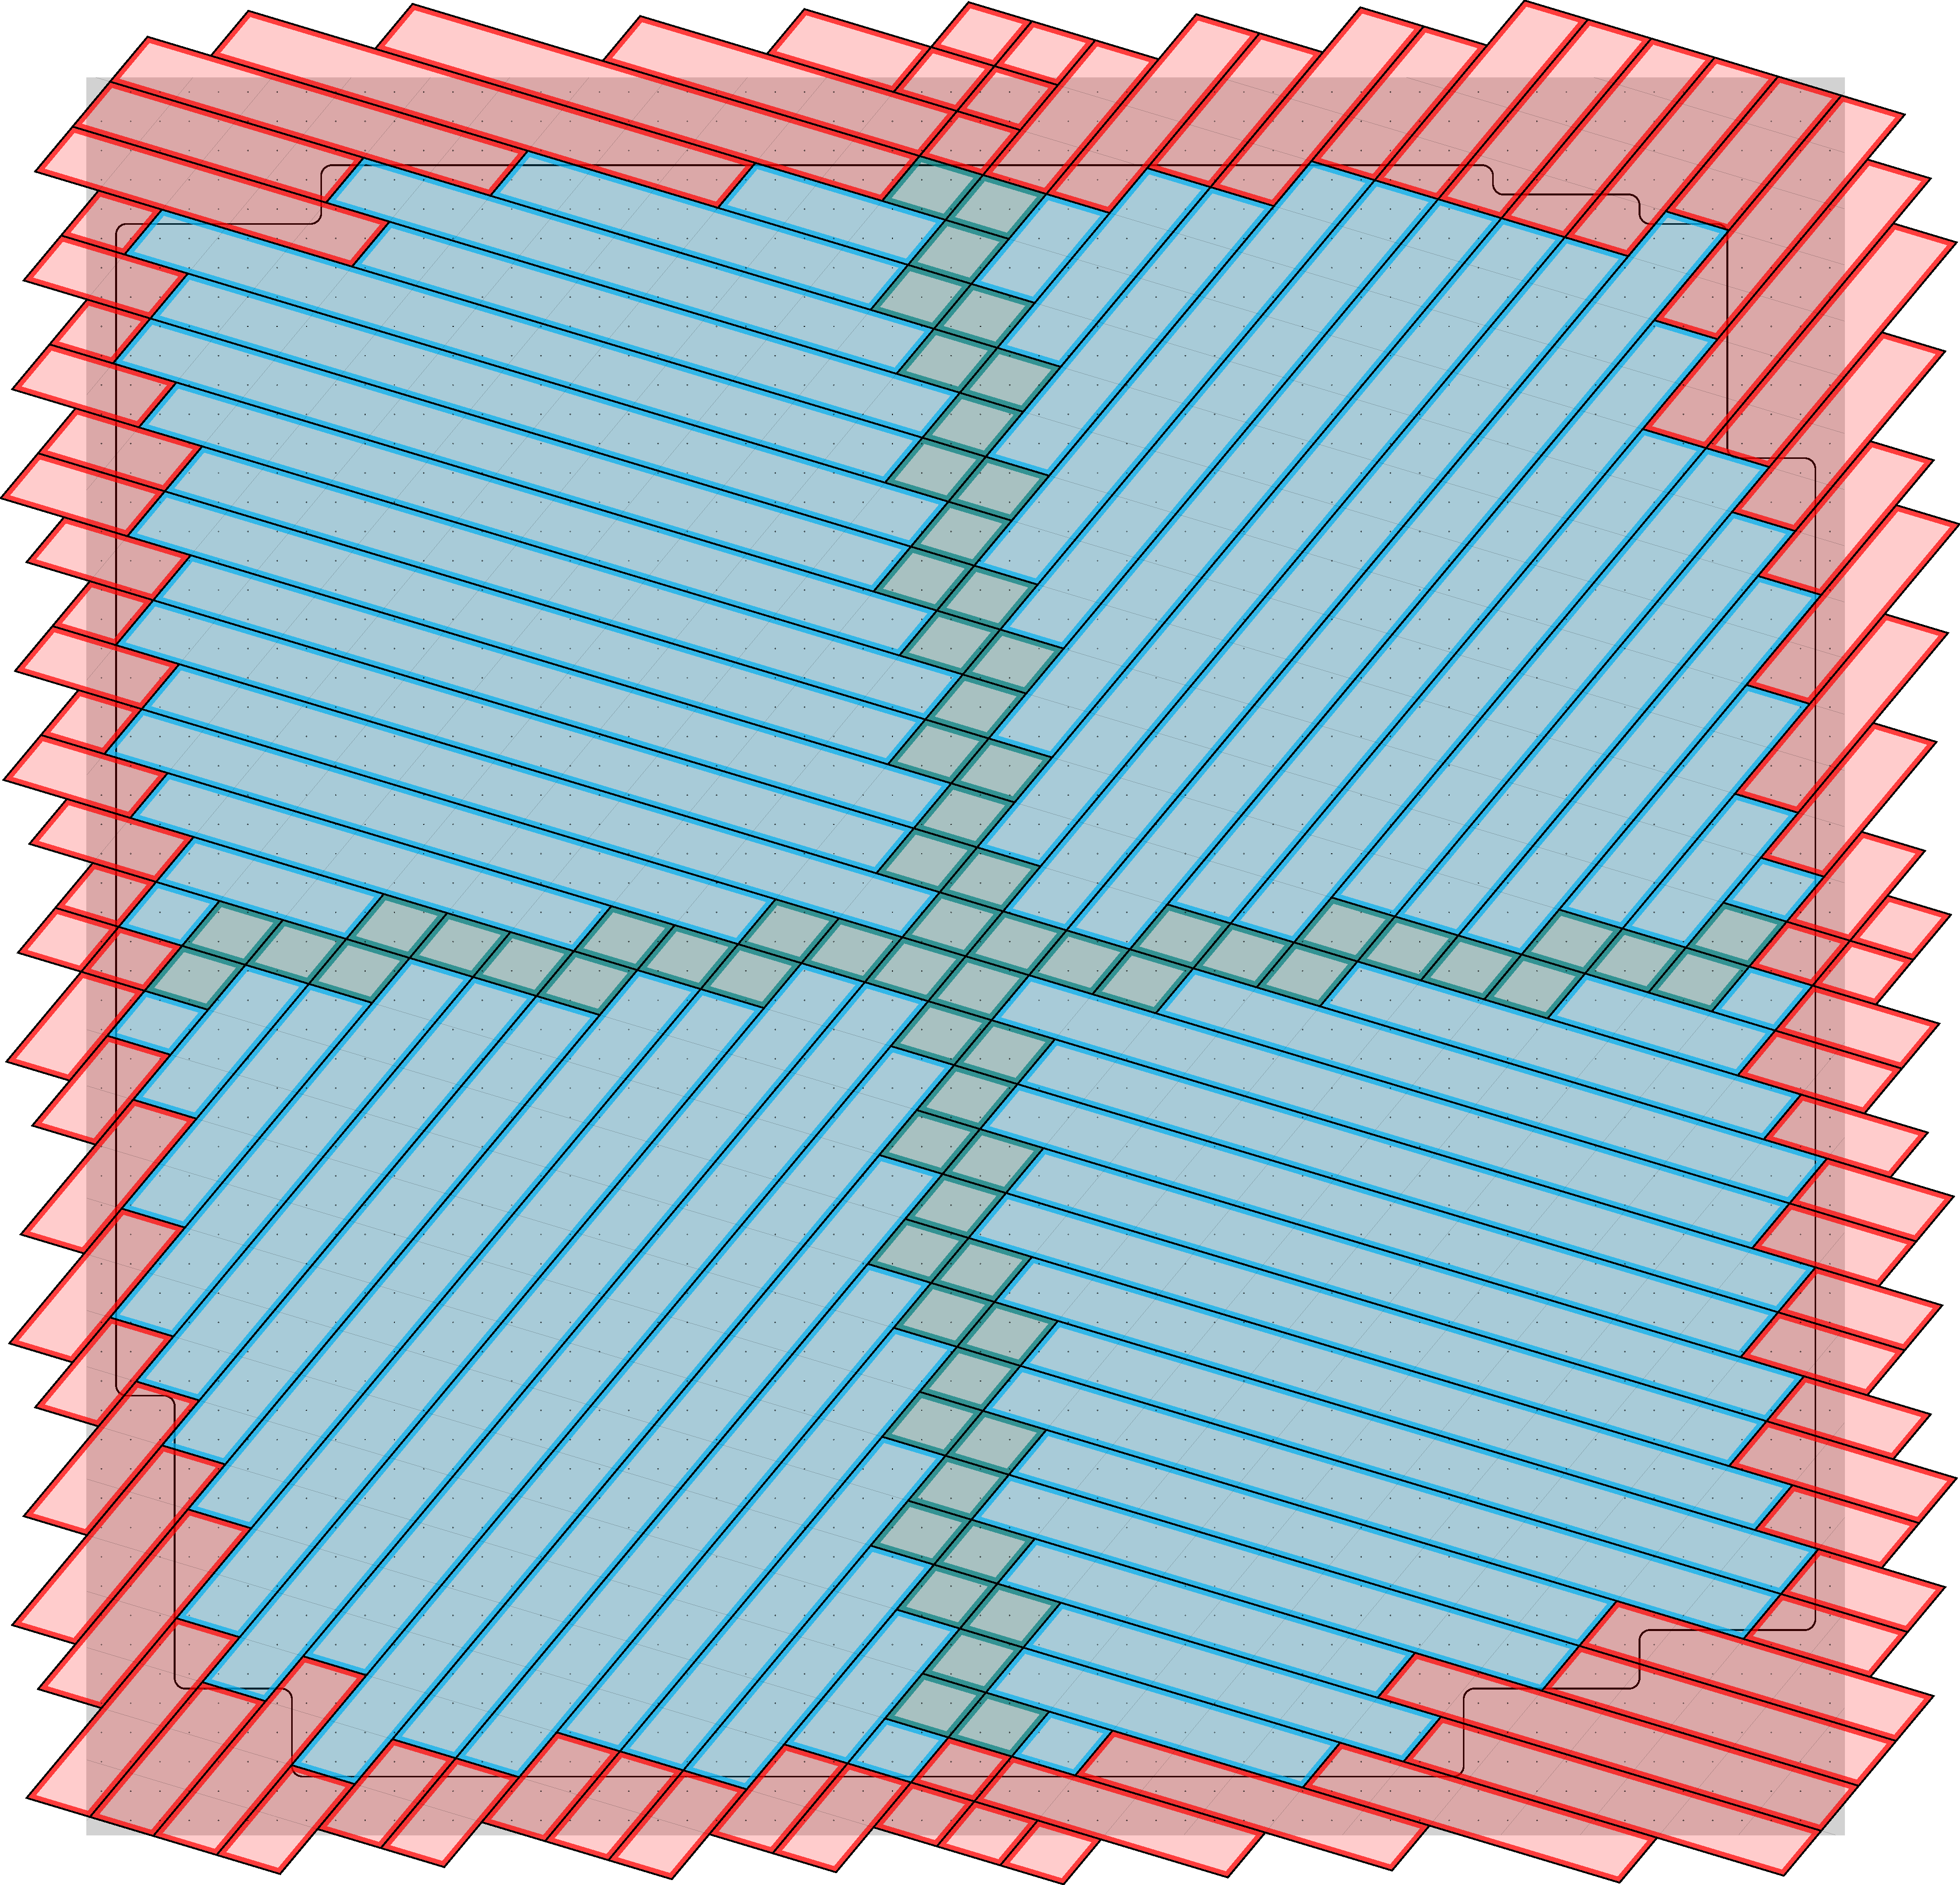
\includegraphics[width=0.8\textwidth]{drawings/text_decomposition}
	\end{center}
	\caption{The parallelograms from $\C$ (blue) and $\C'$ (green).}
	\label{figure:text_decomposition}
\end{figure}

\begin{definition}[Coverability]
	We say that a set $U \subseteq \Z^2$ is \textbf{coverable} if $U \subseteq \d{P + q}$ for some $q \in Q$.
\end{definition}

\begin{lemma}\label{I_division}
	For every $p \in \I$, the set $p \cap \Z^2$ is either coverable or $\O(n / \ell)$-peripheral.
	\begin{proof}
		Consider any $p \in \I$.
		Since the other cases are rotationally symmetric, assume that it intersects with some point $s \in \R^2$, such that $\x{s} = z$ and $\y{s} \ge z$.
		Let $v = (\floor{\max \X(p), \max \Y(p)})$.
		We have $\x{v} \ge \floor{z} = n / 2 - 1$ and $\y{v} \ge \floor{z} = n / 2 - 1$.
		If $v \not \in \Ta$, we can see that by \Cref{distance_bound_lemma},
		$|u - v| = \O(n / \ell)$ for every $u \in p \cap \Z^2$, thus $p$ is $\O(n / \ell)$-peripheral.
		If $v \in \Ta$, there exists $q \in Q$, such that $v \in [m]^2 + q$.
		Consider any $u \in p \cap \Z^2$.
		By the assumption that $\max \X(p) - \min \X(p) < m / 4$ and $\max \Y(p) - \min \Y(p) < m / 4$ we get
		\eq{
			\x{u} \ge n / 2 - m / 4 \ge n - m \ge \x{q},\\ 
			\y{u} \ge n / 2 - m / 4 \ge n - m \ge \y{q},
		}
		and since $\x{u} \le \x{v} \le \x{q} + m - 1$ and $\y{u} \le \y{v} \le \y{q} + m - 1$, we get $u \in [m]^2 + q$, thus $U \subseteq [m]^2 + q$.
	\end{proof}
\end{lemma}

\begin{lemma}\label{coverable is periodic}
	The restriction of $T$ to a coverable set has $\O(k)$-periods $\phi$ and $\psi$.
	\begin{proof}
		Let $R$ denote the restriction. For $q \in Q$, such that $\d{R} \subseteq \d{P + q}$ we have
		\eq{
			\Ham(R + \phi, R) \le \Ham(R + \phi, P + q + \phi) + \Ham(P + q + \phi, P + q) + \Ham(P + q, R) \le \\
			\le \Ham(T, P + q) + \Ham(P + \phi, P) + \Ham(P + q, T) = \O(k)
		}
		and identically $\Ham(R + \psi, R) = \O(k)$.
	\end{proof}
\end{lemma}

\begin{lemma}\label{parallelogram_split_lemma}
	For every $g \in \G$ we can construct two parallelograms $c$ and $b$, such that
	\begin{itemize}
		\item $c \cap \Z^2$ is coverable,
		\item $b \cap \Z^2$ is $\O(n / \ell)$-peripheral,
		\item $g \cap \Z^2$ is partitioned into $b \cap \Z^2$ and $c \cap \Z^2$.
	\end{itemize}
	\begin{proof} See the next section (\ref{parallelogram_split_lemma_proof}). \end{proof}
\end{lemma}

\newcommand{\B}{\mathcal{B}}

We split every non-empty parallelogram $g \in \G$ (by \Cref{parallelogram_split_lemma}) into parallelograms $c$ and $b$.
We construct the set $\C$ consisting of all the obtained parallelograms $c$ and a set $\B$ consisting of all the obtained parallelograms $b$.

We similarly divide the parallelograms in $\I$ (by \Cref{I_division}) and construct the sets $\C' = \set{p : p \in \I, p \cap \Z^2 \text{ is coverable}}$ and $\B' = \I \setminus \C'$.

Now construct $\U = \set{c \cap \Z^2 : c \in \C \cup \C'}$ and $V = \bigcup_{b \in \B \cup \B'} b \cap \d{\Ta}$.
Observe that all sets $U \in \U$ are coverable simple parquets, the set $V$ is $\O(n / \ell)$-peripheral, and $\d{\Ta}$ is partitioned into sets $\U \cup \set{V}$.

The decomposition is illustrated in \Cref{figure:text_decomposition}.
The points in the gray area are outside of the active text.
The parallelograms from $\C$ and $\C'$ are colored blue and green, respectively.
The points outside of them (in the white area) form the peripheral set $V$.

For each $U \in \U$ we construct the restriction of $T$ to $U$.
By \Cref{coverable is periodic}, it has $\O(k)$-periods $\phi$ and $\psi$, thus, by \Cref{parquet_decomposition}, it can be partitioned into $\O(k)$ monochromatic simple subparquet strings.
Since $|\C'| \le |\I| = \O(\ell)$ (by \Cref{I_size_bound}) and $|\C| \le |\G| = \O(\ell)$, we have $|\U| = |\C| + |\C'| = \O(\ell)$, thus the total number of constructed strings is $\O(\ell k)$.

Finally, we construct the restriction of $T$ to $V$, which is a $\O(n / \ell)$-peripheral string.


% PROOF OF SPLIT LEMMA
\subsubsection{Parallelogram splitting} \label{parallelogram_split_lemma_proof}

This section serves as the proof of \Cref{parallelogram_split_lemma}, introduced at the end of the previous section (\ref{text_decomposition_proof}).
Since for an empty parallelogram the proof is trivial, consider a non-empty set $g^1_j$ for some $j \in [\ell]$.
We will explore some properties of the part of the text contained in $K_1$ specifically, which then can be generalized to other quarters by symmetry.

\begin{lemma}\label{coverability_condition}
	Every set $U \subseteq K_1 \cap \Z^2$, such that $(\max \X(U), \max \Y(U)) \in \Ta$ is coverable.
	\begin{proof}
		Let $v = (\max \X(U), \max \Y(U))$.
		By assumption, there exists $q \in Q$, such that $v \in [m]^2 + q$.
		For every $u \in U$ we have
		$\x{q} \le n - m \le n / 2 \le \x{u} \le \x{v} < \x{q} + m$
		and $\y{q} \le n - m \le n / 2 \le \y{u} \le \y{v} < \y{q} + m$,
		thus $u \in [m]^2 + q$.
	\end{proof}
\end{lemma}

\begin{observation}\label{domination_lemma}
	By \Cref{coverability_condition}, there does not exist a pair of points $u \in \Z^2 \cap K_1 \setminus \d{\Ta}$ and $v \in \Ta$, such that $\x{u} \le \x{v}$ and $\y{u} \le \y{v}$. 
\end{observation}

Recall that there exists $t \in [\ell + 1]$, such that
$ g^1_j = \bigcup_{i = t}^{\ell - 1} p_{i, j}.$
We find 
\[ f = \min\set{i : i \in \set{t, \dots, \ell - 1}, (\floor{\max \X(p_{i, j})}, \floor{\max \Y(p_{i, j})}) \in \Z^2 \setminus \d{\Ta}}.\]
If the minimum does not exist, we consider $f = \ell$.
We then construct the parallelograms
\[c = \bigcup_{i = 0}^{f - 1} p_{i, j}, \quad b = \bigcup_{i = f}^{\ell - 1} p_{i, j}.\]

We now show that the set $c \cap \Z^2$ is coverable.
If $c \cap \Z^2$ is empty, then it is coverable, so let us assume it is not.
In that case $f > 0$.
It is clear that $c \cap \Z^2 \subseteq K_1$.
By \Cref{monotonicity_lemma}, we have 
\eq{
	\max \X(c) = \max \X(p_{f - 1, j}), \\
	\max \X(c) = \max \Y(p_{f - 1, j}),
}
and thus
\eq{
	\max \X(c \cap \Z^2) &\le \floor{\max \X(c)} = \floor{\max \X(p_{f - 1, j})}, \\
	\max \Y(c \cap \Z^2) &\le \floor{\max \Y(c)} = \floor{\max \Y(p_{f - 1, j})}.
}

We see that $(\max \X(c \cap \Z^2), \max \Y(c \cap \Z^2)) \in \Ta$, since it would otherwise contradict \Cref{domination_lemma},
considering that
$(\floor{\max \X(p_{f - 1, j})}, \floor{\max \Y(p_{f - 1, j})}) \in \Ta$.
We see that $c \cap \Z^2$ satisfies the conditions of \Cref{coverability_condition}, thus $c \cap \Z^2$ is coverable.

We now show that the set $b \cap \Z^2$ is $\O(n / \ell)$-peripheral.
If it is empty, then the proof is trivial, so let us assume it is not.
In that case $f < \ell$.
Denote $v = (\floor{\max \X(p_{f, j})}, \floor{\max \Y(p_{f, j})})$.
By definition, $v \in \Z^2 \setminus \d{\Ta}$.
Consider any point $u \in b \cap \Z^2$.
There exists exactly one $i \in \set{f, \dots, \ell - 1}$, such that $u$ lays strictly inside $p_{i, j}$.
Let $w = (\floor{\max \X(p_{i, j})}, \floor{\max \Y(p_{i, j})})$.
By \Cref{monotonicity_lemma}, we have $\x{w} \ge \x{v}$ and $\y{w} \ge \y{v}$, and by considering \Cref{domination_lemma},
we get $w \in \Z^2 \setminus \d{\Ta}$.
Finally, by \Cref{distance_bound_lemma}, we get $|u - w| = \O(n / \ell)$.

The constructions for $g^2_i$, $g^3_j$, $g^4_i$ are rotationally symmetric.


% PROOF OF DISTANCE BOUND
\subsubsection{Parallelogram span bounds} \label{distance_bound_lemma_proof}

In this section we will establish a distance bound for points laying inside or in the proximity of the constructed parallelograms.
Consider any fixed $p_{i, j}$ for some $i, j \in [\ell]$.
We first show some auxiliary (weaker) lemmas, which we then use to prove \Cref{distance_bound_lemma}.

\begin{lemma}\label{distance_bound_aux}
	For every $u, v \in p_{i, j}$, we have $|u - v| = \O(n / \ell)$.
	\begin{proof}
		Consider any $u, v \in p_{i, j}$ and denote $w = u - v$.
		By definition of $p_{i, j}$, we have
		\[ |\h{w}| = |\h{(u - v)}| = |\h{u} - \h{v}| = \O(n|\phi| / \ell) \]
		and similarly $|\s{w}| = \O(n|\psi| / \ell)$.
		Since $\phi$ and $\psi$ are not colinear, there exist $s, t \in \mathbb{R}$, such that $w = s\phi + t\psi$.
		Recall that by \Cref{get_periods} we have $|\phi \times \psi| \ge \frac{1}{2}|\phi||\psi|$ (since $|\sin \alpha| \ge 1/2$), thus
		\[ \frac{1}{2}|t||\phi||\psi| \le |t||\phi \times \psi| = |\phi \times (s\phi + t\psi)| = |\h{w}| = \O(n|\phi| / \ell), \]
		which gives us $|t\phi| = \O(n / \ell)$.
		We can similarly prove that $|s\psi| = \O(n / \ell)$ and finally
		\[ |w| = |s\phi + t\psi| \le |s\phi| + |t\psi| = \O(n / \ell). \]
	\end{proof}
\end{lemma}

\begin{lemma}\label{distance_bound_aux2}
	For every point $u \in \X(p_{i, j}) \times \Y(p_{i, j})$ there exists a point $v \in p_{i, j}$, such that $|u - v| = \O(n / \ell)$.
	\begin{proof}
		There exists a point $w \in p_{i, j}$, such that $\x{u} = \x{w}$, and a point $v \in p_{i, j}$, such that $\y{u} = \y{v}$.
		By \Cref{distance_bound_aux}, we have
		\[|u - v| = |\x{u} - \x{v}| = |\x{w} - \x{v}| \le |w - v| = \O(n / \ell).\] 
	\end{proof}
\end{lemma}

\DistanceBoundLemma
\begin{proof}
	Consider any $u, v \in p_{i, j}$.
	By \Cref{distance_bound_aux2}, there exist $u', v' \in p_{i, j}$ such that $|u - u'| = \O(n / \ell)$ and $|v - v'| = \O(n / \ell)$.
	By \Cref{distance_bound_aux}, we have
	\[ |u - v| \le |u - u'| + |u' - v'| + |v' - v| = \O(n / \ell). \]
\end{proof}

\bibliographystyle{plainurl}
\bibliography{references}

\end{document}

